

\documentclass[
	11pt, % Set the default font size, options include: 8pt, 9pt, 10pt, 11pt, 12pt, 14pt, 17pt, 20pt
	%t, % Uncomment to vertically align all slide content to the top of the slide, rather than the default centered
	%aspectratio=169, % Uncomment to set the aspect ratio to a 16:9 ratio which matches the aspect ratio of 1080p and 4K screens and projectors
]{beamer}

\graphicspath{{img/}} 
\usepackage{amsmath} % for math formatting
\usepackage{booktabs} 

\usepackage{multirow}
\usepackage{multicol}

\usepackage{colortbl}
\usepackage{xcolor}
\usepackage{tcolorbox}


\usetheme{Boadilla}

\usecolortheme{whale}    


\usefonttheme{default} 

\usepackage{palatino} 


\usepackage[default]{opensans} 

\useinnertheme{circles}

\useoutertheme{miniframes}


\title[Demographics of Unemployment: An inspection through Covid-19]{Demographics of Unemployment: An inspection through Covid-19} 

\author[EC48K \\ Can Portakal, Zeynep Bozoklu]{{\small EC48K\\ Can Portakal\\Zeynep Bozoklu}}


\institute[BOUN]{Bogazici University} 

\date[Dec 13, 2024]{\Small Dec 13, 2024} 


\begin{document}

\begin{frame}
    \centering
    % Place the logo at the top
    
\includegraphics[width=1.8cm]{BOUN.png} % Adjust width to make the logo smaller
    \vspace{0.1cm} % Space between logo and title
    \titlepage

\end{frame}


\section{Introduction}

\begin{frame}

    \frametitle{Introduction}

    \begin{itemize}
        \item Covid-19 was a prominent crisis that had serious impact on many aspects of our societies.

        \item Starting from the 17th November 2019 in Wuhan, China; it had a chain impact on societies in terms of humanitarian, social and economic aspects.
    \end{itemize} 
    
    
\end{frame}

\begin{frame}

    \frametitle{Introduction(cont'd)}
    \begin{itemize}
        \item Obviously, the contagious nature of the disease had a serious impact on people to avoid getting together to transact, consume and more importantly, to produce; which all led to a shrinking in total economic activity.
        \item  This shrinkage of economic activities in countries with the Covid-19 cases has led to a global economic recession.
        
    \end{itemize}
    
    \end{frame}

\begin{frame}
   \frametitle{Some Facts and Figures}
    \begin{itemize}
        \item The International Labour Organization (ILO) estimated a loss of 255 million full-time jobs in 2020, approximately four times greater than during the 2009 global financial crisis.
        \item The global economy contracted by about 3.4\% in 2020, marking the worst peacetime recession since the Great Depression.
        \item Global tourism revenues fell by 72\% in 2020, with a slow recovery thereafter.
    \end{itemize}
    
    

\end{frame}

\section{Motivation}
\begin{frame}
    \frametitle{Why study unemployment demographics?}
     \begin{itemize}
        \item[$\rightarrow$]  Now, it is obvious that COVID had an impact on almost anything in our lives. Then why do we specifically study labor market and unemployment dynamics across demographic groups during COVID-19?
     
        \end{itemize}
    
      
\end{frame}

\begin{frame}
    \frametitle{Why study unemployment demographics?(cont'd)}
        \begin{itemize}
            \item[$\rightarrow$] \small Unemployment directly affects \textbf{income, consumption}, and overall economic stability.
            
            \item[$\rightarrow$] \small The pandemic exacerbated existing inequalities; hitting \textbf{low-wage workers, minorities,} and \textbf{women} particularly hard. Low-wage and minority workers experienced higher unemployment rates, and women faced increased caregiving burdens, potentially leading to long-term effects for their labor market attachment and wage growth. \textcolor{blue}{(Piacentini, Frazis et al., 2022)}
            
            \item[$\rightarrow$] \small Understanding labor market impacts is essential for designing effective interventions, such as targeted support for vulnerable groups, retraining programs, and reforms to address systemic disparities. \textcolor{blue}{(Hershbein, Holzer 2021)}   
        \end{itemize}
\end{frame}


\begin{frame}{Why study unemployment demographics in Turkey?}
    \begin{itemize}
        \item[$\rightarrow$] The first positive-tested case in Turkey was seen on March 11th, 2020 in Istanbul.
        \item[$\rightarrow$] The first death because of COVID was declared on March 15th, 2020.
        
    \end{itemize}
    
    
\end{frame}


\begin{frame}{Why study unemployment demographics in Turkey?(cont'd)}
    \begin{itemize}
        \item Schools and universities were closed on March 16, 2020, and public events were suspended. 
        \item Turkey imposed travel bans on 68 countries: like China,  Germany, France...etc.
        \item A curfew was imposed on individuals over 65 and those under 20. Weekend and public holiday lockdowns were implemented in many cities.
        
        \item Some of the industrial giants of Turkey, such as Ford Otosan, Toyota and Hyundai announced that they will suspend production in their factories at Kocaeli, Gölcük and Sakarya. 

    \end{itemize}

    
\end{frame}

\begin{frame}{Why study unemployment demographics in Turkey? (cont'd)}
\begin{itemize}
    \item  Although advanced economies shrank by 4.5\%, while emerging markets and developing economies faced a 2.1\% contraction on average, \textbf{Turkey's real GDP grew by 1.8\% in 2020.} This growth rate was \textbf{the second-highest among G20 countries}, surpassed only by China.
    \item  The unemployment rate in Turkey stood at 13.2\% in 2020, highlighting significant labor market pressures despite government support programs.
    

\end{itemize}
\end{frame}

\begin{frame}{Why study labor market in Turkey? (cont'd)}
\begin{itemize}
    \item Turkey implemented a large-scale \textbf{economic stimulus package, equivalent to about 12\% of GDP}, including credit guarantees, tax deferrals, and low-interest-rate policies, which helped mitigate the economic downturn.
    \item In terms of the policy measures adopted during the pandemic, an aggressive easing policy based on sizable bond purchases and credit growth was implemented during the first half of the year. \textcolor{blue}{(Demiralp, Çakmaklı, 2020)}
    \item According to data from the Central Bank of the Republic of Türkiye (CBRT), credit growth exceeded 50\% in real terms, one of the highest rates globally during this period.
    
\end{itemize}
      
\end{frame}




\begin{frame}{Timeline}
    \scriptsize 
    \begin{table}
        \centering
        \begin{tabular}{|c|c|}
            \hline
            \textcolor{blue}{Date}   & \textcolor{blue}{Event} \\ \hline
            \textbf{March 11th}    &  \textbf{First case detected} \\ \hline
            March 16th    & Public places closed \\ \hline
            March 19th    & \$15 billion economic stimulus package \\ \hline
            March 21th    & Nationwide curfew \\ \hline
            March 30th    & Entrance to major cities banned \\ \hline
            \textbf{April 3th} & \textbf{Major Lockdown} \\ \hline
            April 28th   & Short-term work permits \\ \hline
            May 5th    & Reopening of automotive factories \\ \hline
            May 17th    & Cash assistance programs \\ \hline
            \textbf{June 1st}   & \textbf{Restrictions began easing} \\ \hline
            \textbf{November 20th} & \textbf{Reintroduction of restrictions} \\ \hline
            \textbf{March 2021} & \textbf{Temporary easing of restrictions} \\ \hline
            \textbf{April 29th 2021 }   & Full lockdown \\ \hline
            June 2021    & Gradual reopening \\ \hline
        \end{tabular}
        \caption{Timeline of COVID-19 Pandemic in Türkiye}
    \end{table}
\end{frame}

\begin{frame}{Objectives}      
   
    \begin{exampleblock}{}
        \begin{itemize}
	        \item \small We try \textbf{to assess and quantify how heterogenous was the economic impact of COVID-19 on different demographic groups}  in Turkey, by using recent cross-section and panel data of TurkStat.

            \item \small Providing a descriptive analysis by tracking specific individuals and households captured by \textbf{SILC Panel Data of TurkStat between 2018-2021.}
            \item \small \textbf{Rigorous analysis using the latest data} needed to understand why the pandemic in Turkiye has been very unequal in terms of its impact on different groups, which is a factor that is affecting many aspects in terms of policy making or social life and to come up with realistic and efficient policy making suggestions.
	    \end{itemize}
    \end{exampleblock}

    \end{frame}

\begin{frame}
    \frametitle{Cross-Section}
    \begin{figure}
        \centering
        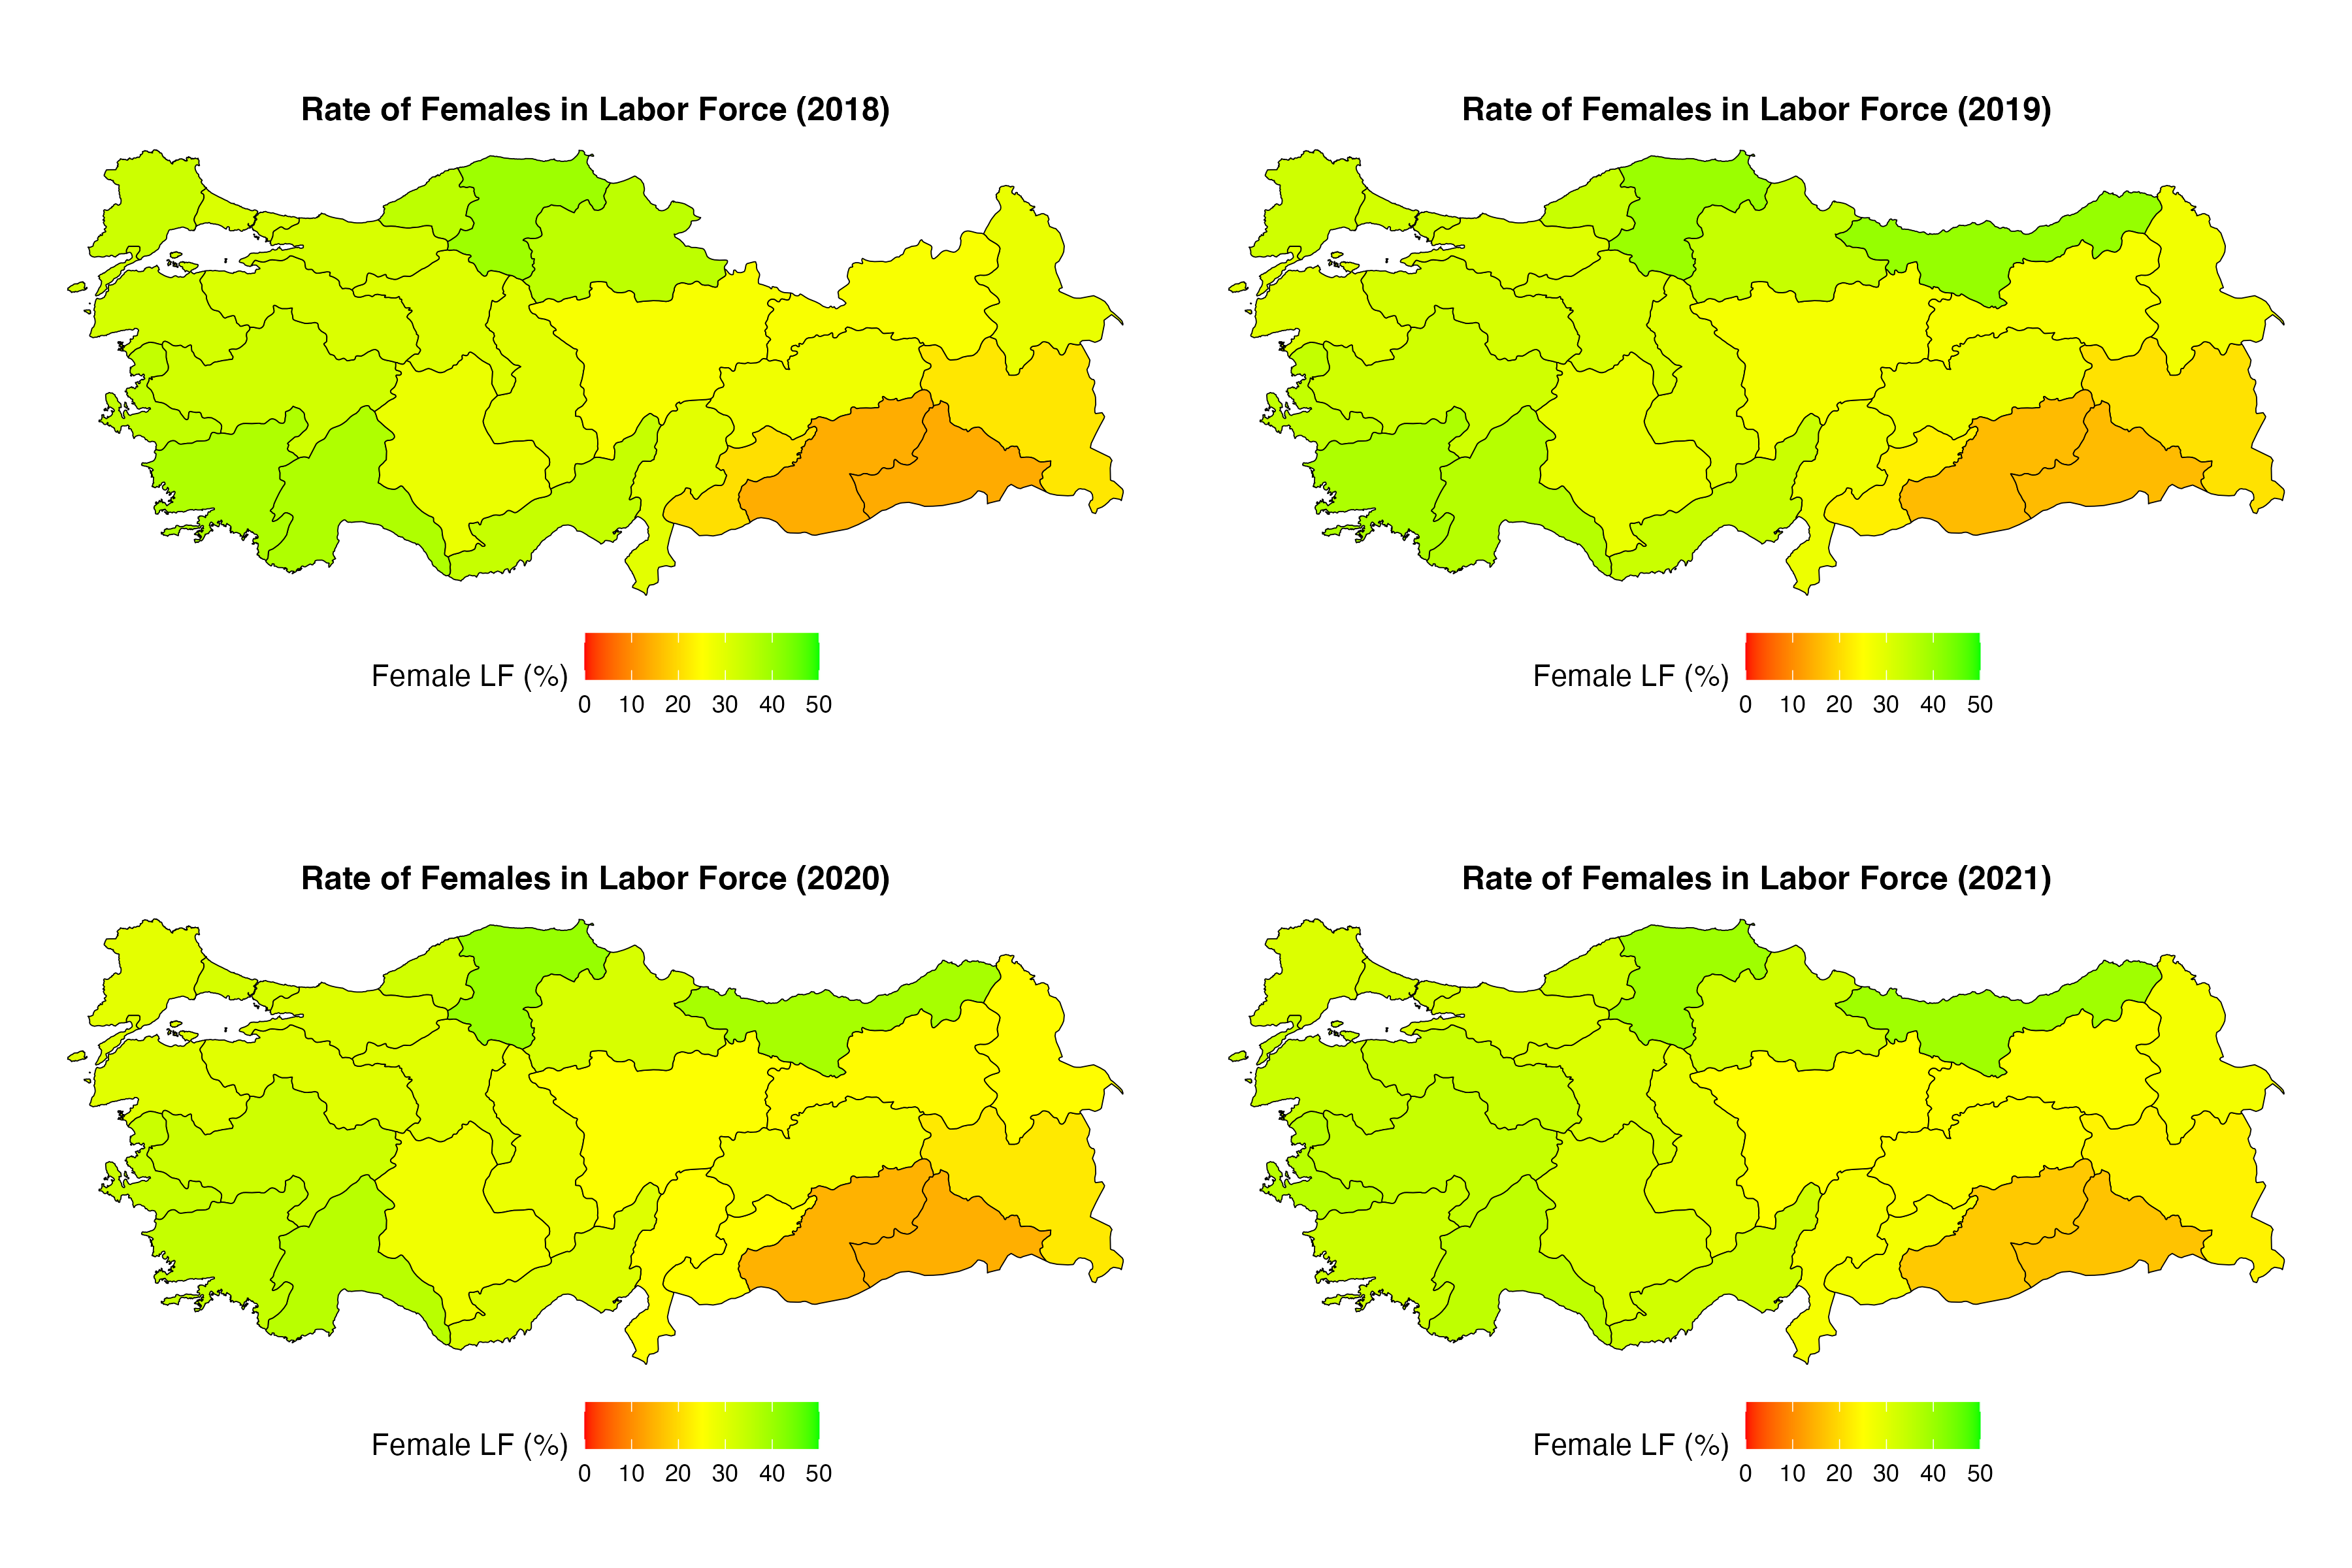
\includegraphics[width=0.75\linewidth]{female_lf_maps_2018_2021.png}
        \caption{Rate of Females in Labor Force}
        \label{fig:female_lf}
    \end{figure}
\end{frame}

\begin{frame}
    \frametitle{Cross-Section}
    \begin{figure}
    \centering
    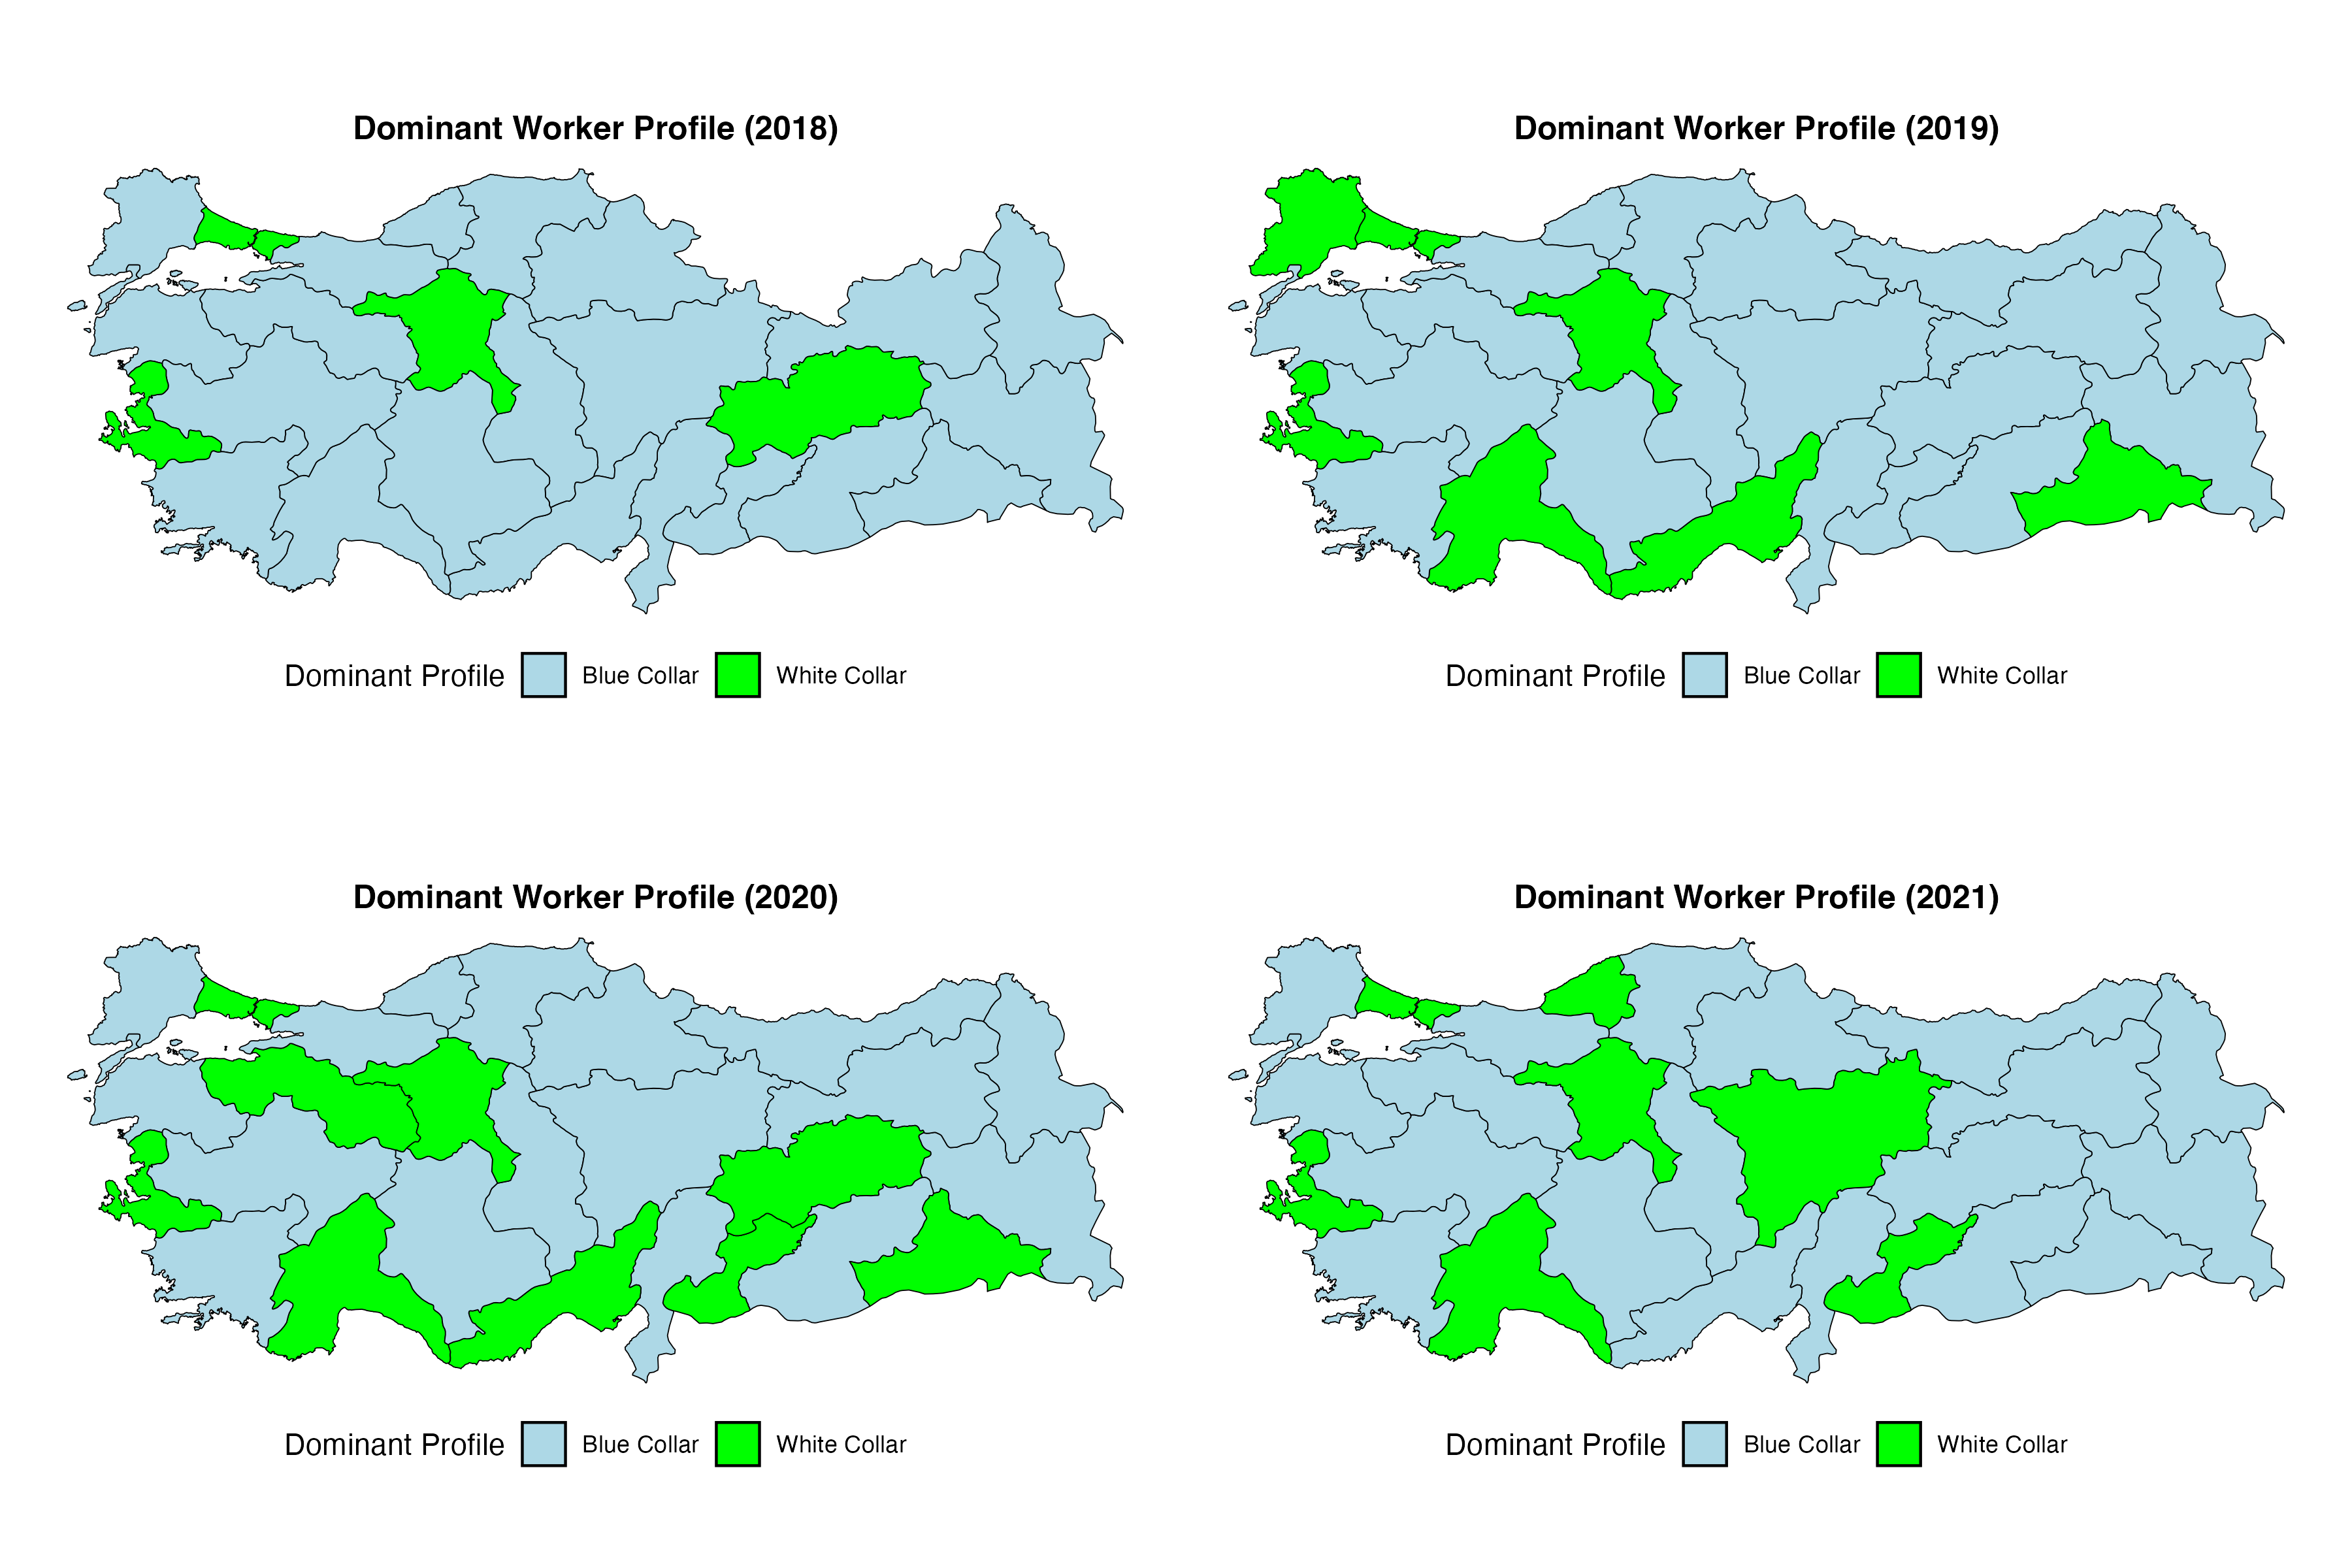
\includegraphics[width=0.75\linewidth]{dominant_worker_profiles_2018_2021.png}
    \caption{Dominant Worker Profiles in Labor Force}
    \label{fig:domworker_lf}
\end{figure}
\end{frame}

\begin{frame}
    \frametitle{Cross-Section}
    
\begin{figure}
    \centering
    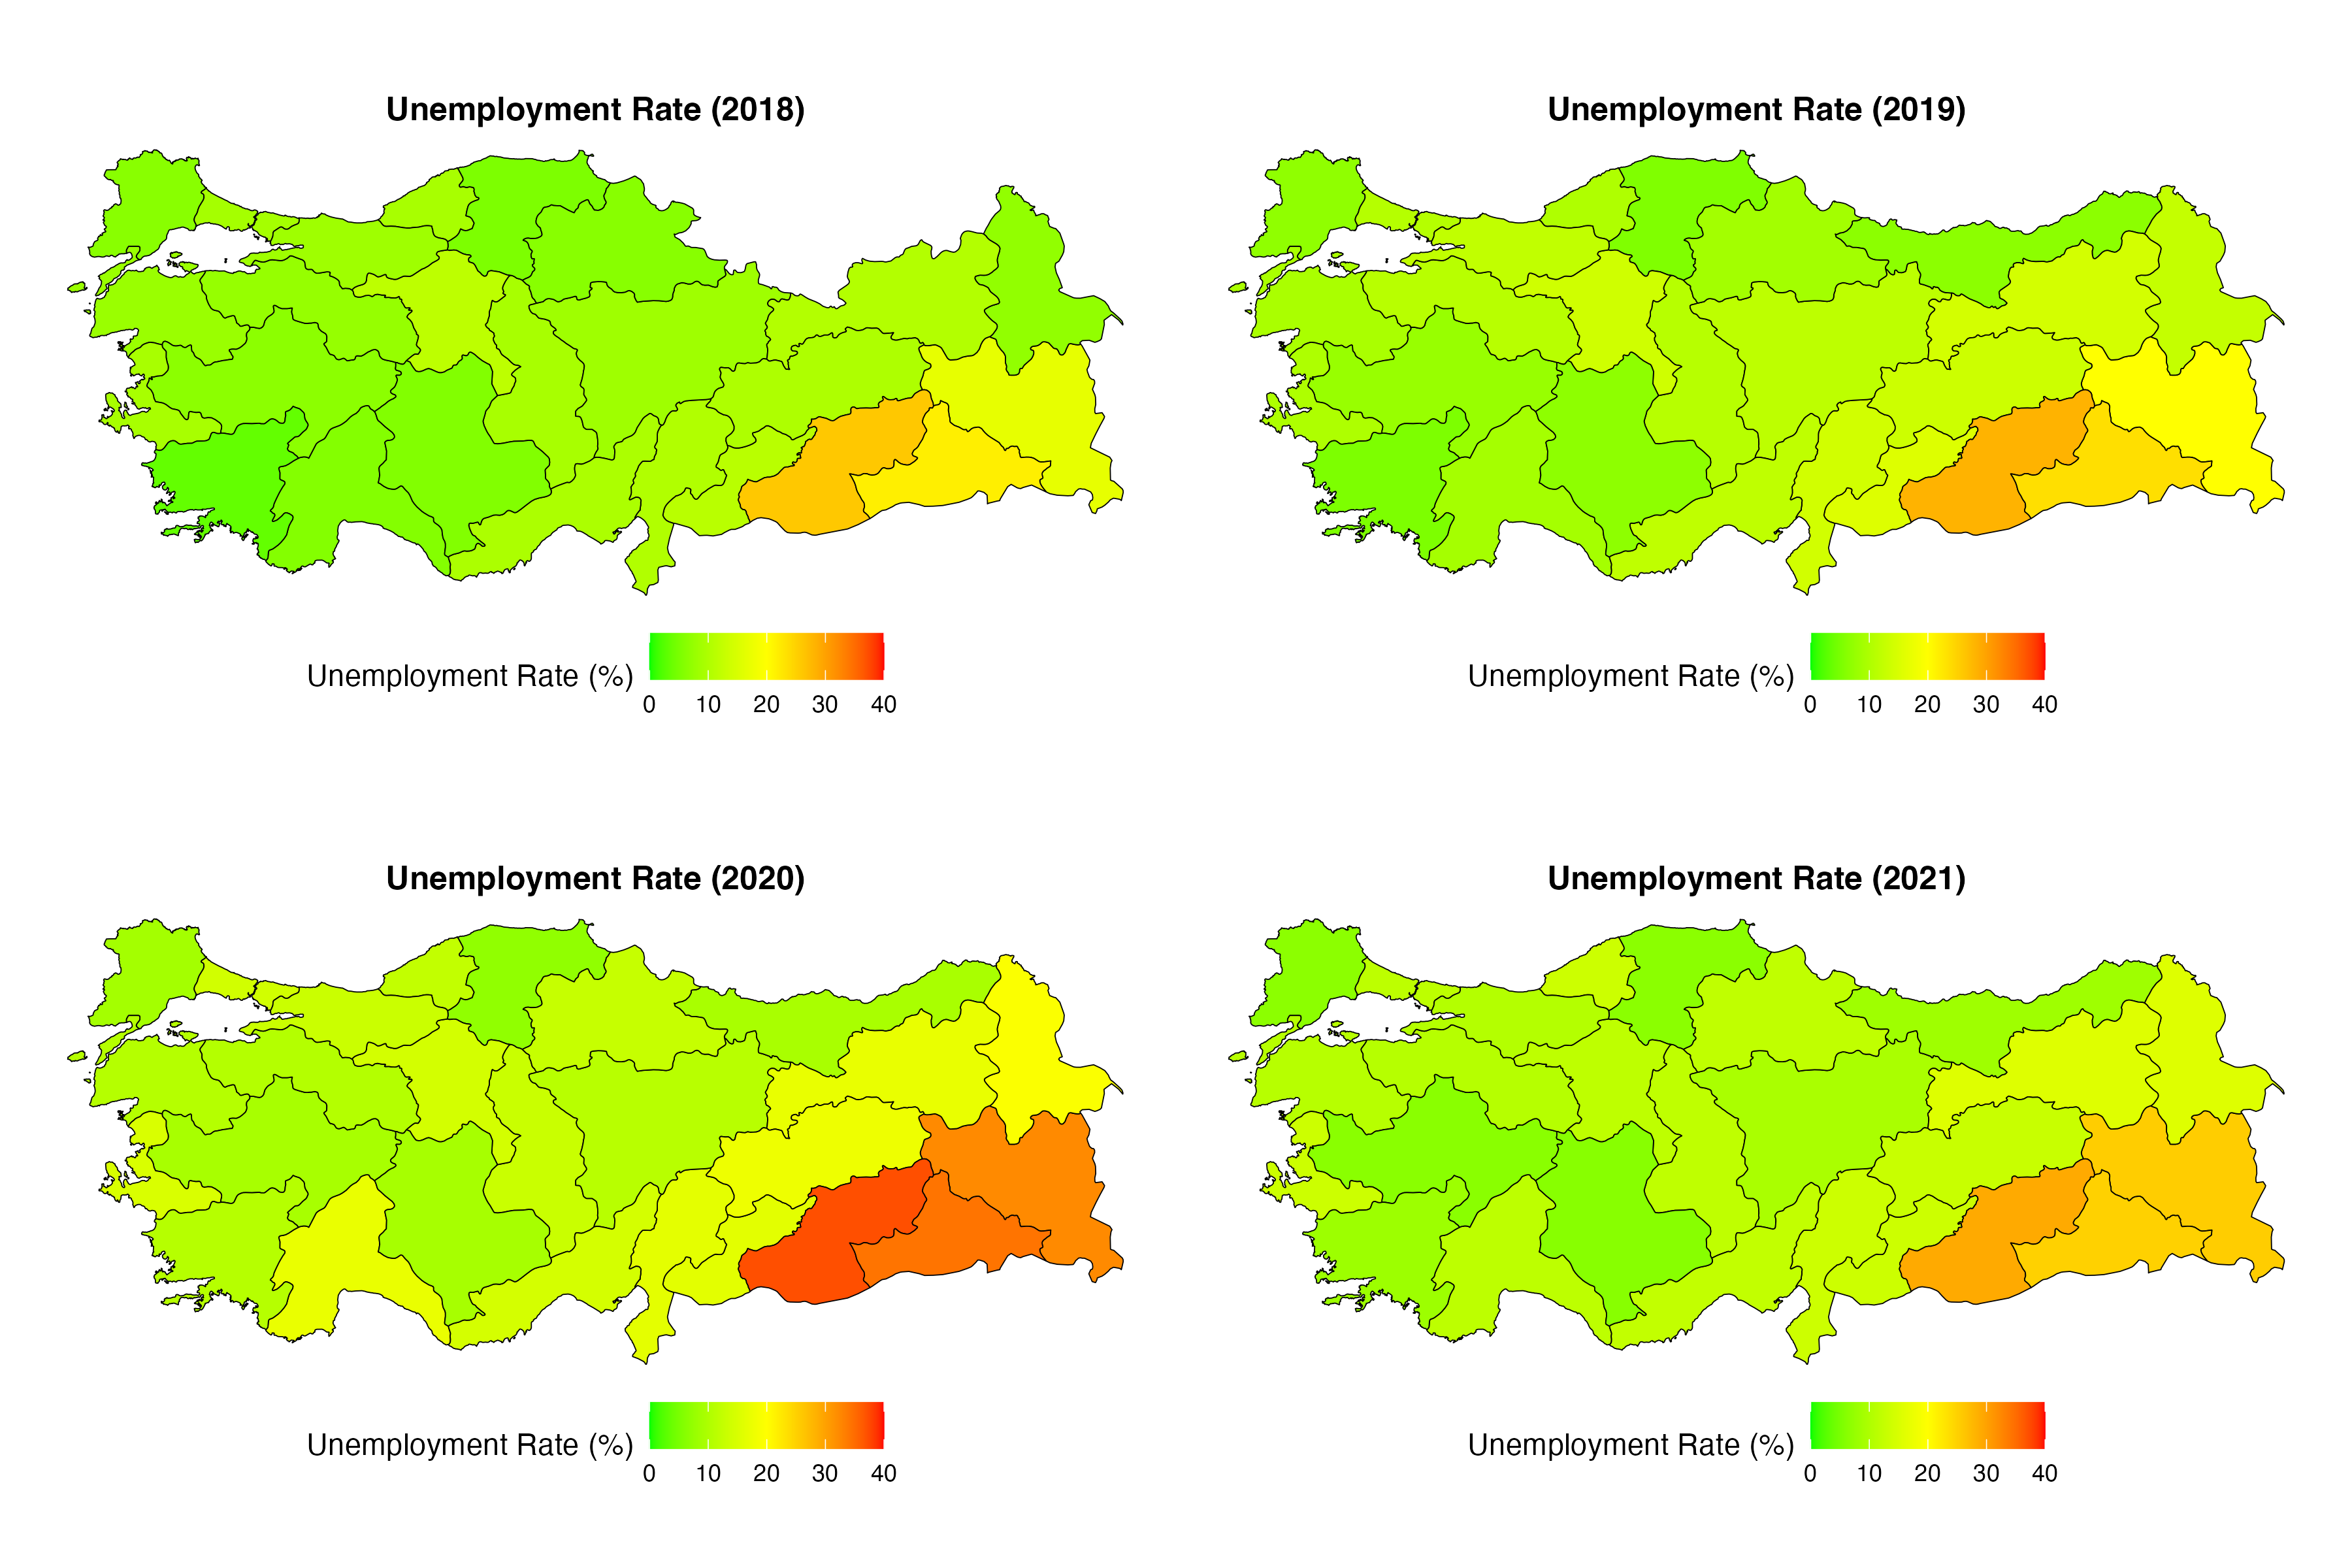
\includegraphics[width=0.75\linewidth]{unemployment_maps_2018_2021.png}
    \caption{Unemployment Rates}
    \label{fig:unemp_rates}

\end{figure}

\end{frame}

\begin{frame}
    \frametitle{Cross-Section}
    \begin{figure}
    \centering
    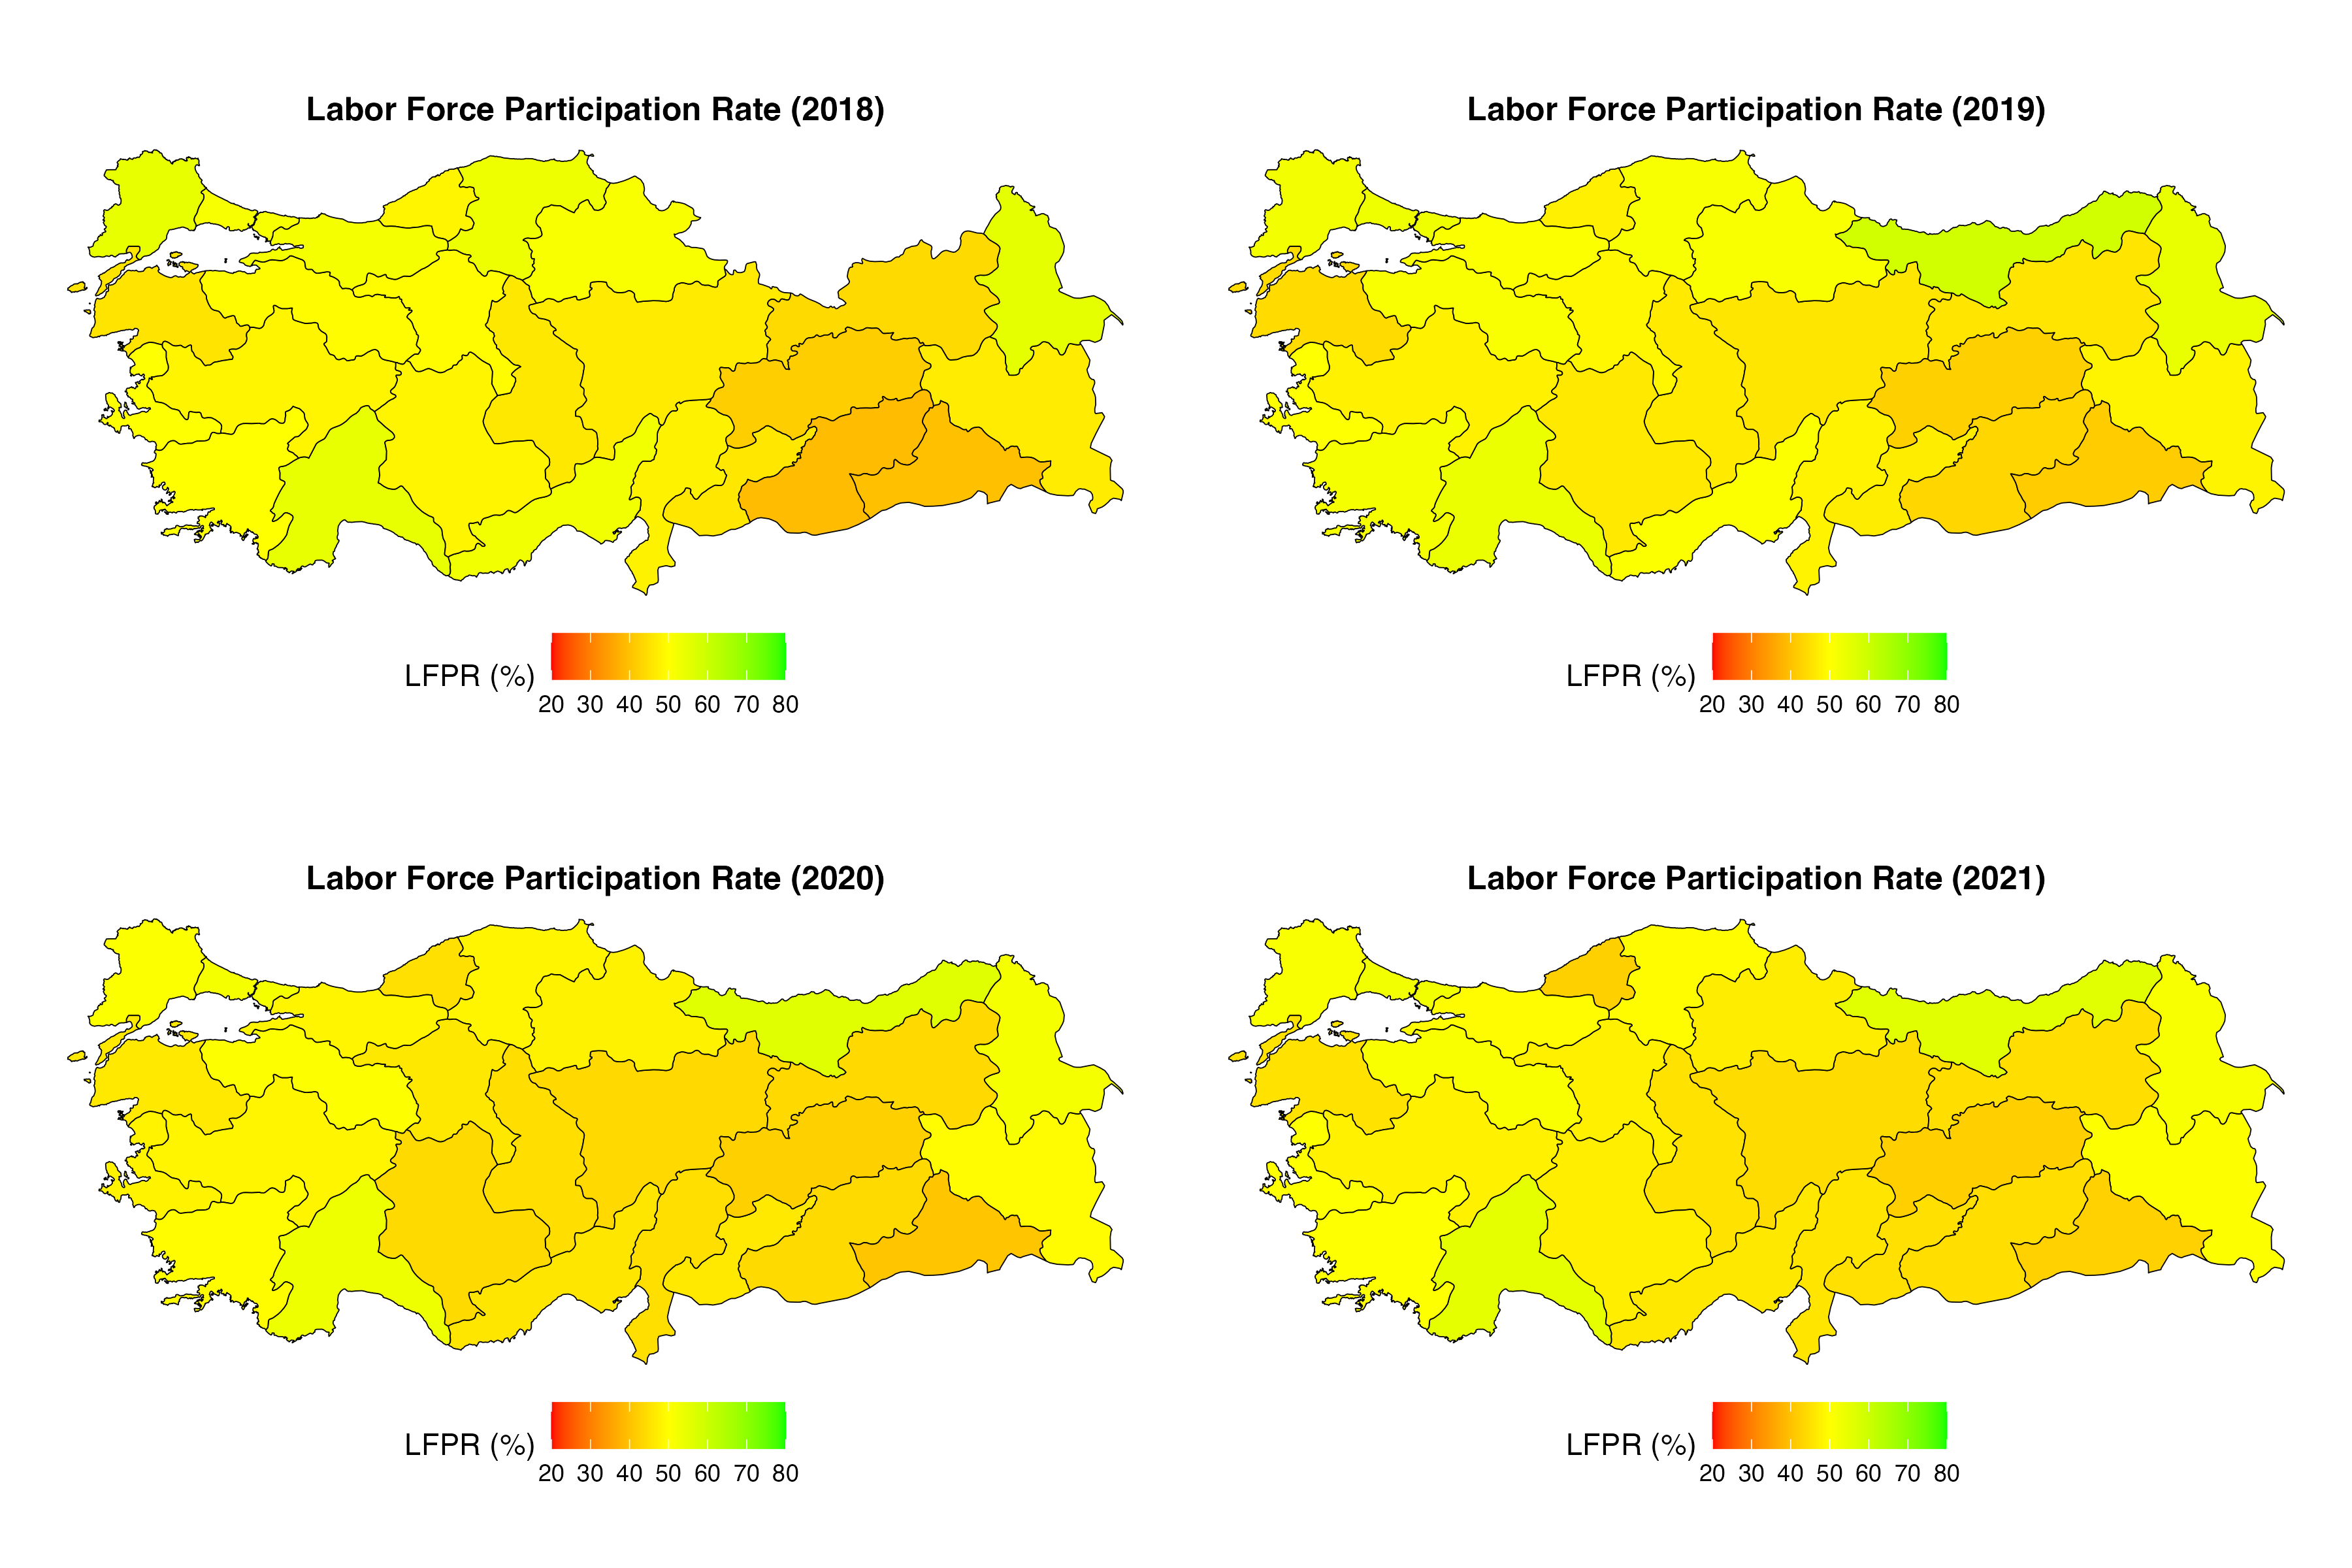
\includegraphics[width=0.75\linewidth]{lfpr_maps_2018_2021.png}
    \caption{Labor Force Participation Rates}
    \label{fig:lfpr}
\end{figure}
\end{frame}




\section{Literature Review}
\begin{frame}
    \frametitle{Literature Review}
        \begin{itemize} 
            \item[$\rightarrow$] \textcolor{blue}{(Aygün et al. 2021)} report that women who have children and do not have a high school degree constitute the most vulnerable group  against unemployment and income losses. 

             \item[$\rightarrow$] However, among the university degree holders, the detrimental labor market effects of having children or being a woman are smaller.\textcolor{blue}{(Aygün et al. 2021)}
           
            \item[$\rightarrow$] Same study depicts that men’s unemployment rate \textbf{increased from 12.4 percent to 13.8 percent} between March and July 2020. 
            \begin{itemize}
                \item The employment protection policies were effective in keeping unemployment rate under control for men.
                \item Some men exited the labor force.
            \end{itemize} 

        \end{itemize}   
    
    
\end{frame}

\begin{frame}

    \frametitle{Literature Review}
    \begin{itemize}
        \item  Women’s unemployment rate decreased in the first couple of months of the pandemic but returned to its pre-pandemic rate in July. \textcolor{blue}{(Aygün et al. 2021)}
        \item It is the result that the likelihood of income loss among different groups, the probability of income loss was higher among singles, women, the informally employed, less educated, individuals who live with children or the self-employed. \textcolor{blue}{(Aygün et al. 2021)}
    \end{itemize}
\end{frame}


\begin{frame}

    \frametitle{Literature Review}
    \begin{itemize}
        \item[$\rightarrow$]The least educated were more negatively affected by the pandemic. \textcolor{blue}{(Aldan et al. 2021)}
        \item[$\rightarrow$] \textcolor{blue}{Aum et al. (2021)} show that employment losses due to pandemic in South Korea did not cause an increase in the unemployment rate due to the fall in labor force participation.
        \item[$\rightarrow$] The Covid-19 pandemic has a disproportionate impact on women's socioeconomic outcomes (Brodeur et al., 2021). 
        \begin{itemize}
            \item In order to emphasize this peculiarity of the Covid-19 recession, the term \textit{"shecession”} has been introduced in policy discussions.
        \end{itemize}
        
        
    \end{itemize}
    
    
\end{frame}
\begin{frame}{Literature Review}
\begin{itemize}
    \item Mixed empirical evidence about "shecession".
    \begin{itemize}
        \item[$\rightarrow$] \textcolor{blue}{Cortes and Forsythe(2020)} for the US, \textcolor{blue}{Farre et al.(2020)} for Spain find that women were hurt more in the labor market compared to men. 
        \item[$\rightarrow$] Some others do not find any differential effect such as \textcolor{blue}{Milovanska-Farrington (2021)}  for the US and \textcolor{blue}{Hupkau and Petrongolo (2020)} for the UK. 
    \end{itemize}
\end{itemize}

\end{frame}


\begin{frame}{Literature Review}
     \begin{itemize}
         \item Young are expected to be hurt more since workers with tenure contracts keep their jobs and new entrants into the labor market are severely affected by the decline in the hiring rate \textcolor{blue}{(Hoynes et al., 2012)(Crossley et al. (2021)} .
     \end{itemize}

\end{frame}

\begin{frame}{Literature Review}
    \begin{itemize}
        \item \textcolor{blue}{(Hoehn-Velasco et al.2021)}find that youngest and oldest workers were more affected compared to middle-aged workers in Mexico. 
        \item \textcolor{blue}{(Cortes and Forsythe 2020)}for the US find that less educated were disproportionately affected by the pandemic.
        \item \textbf{On the other hand}, \textcolor{blue}{(Montenovo et al. 2020)} find an inverse U-shaped pattern, meaning that higher educated workers could continue their jobs remotely and least educated workers were concentrated in essential industries where lockdown measures were not implemented.
    \end{itemize} 

 
\end{frame}


\begin{frame}{Literature Review}
\begin{itemize}
    \item In terms of age, \textcolor{blue}{(Aldan et al. 2021)} find a similar \textbf{U-shaped pattern} to that of US; the impact of the pandemic was hardest across young (aged 15-24) and old (55+). 
\end{itemize}
 
    
\end{frame}

\begin{frame}

    \frametitle{Literature Review}
    \begin{itemize}
        \item \textit{Distributed Lag Autoregressive Model} used in \textcolor{(ILO, 2021}){} to assess the impacts of COVİD on different demographics and age groups using pre-covid data.
        \item \textcolor{blue}{(Jackson, 2015)} used \textbf{compositional analysis method} for measuring unemployment. This method will be crucial to our analysis.
    \end{itemize}
    
    
    
\end{frame}

\section{Data}

\begin{frame}

    \frametitle{Data Sources}
    \textbf{Turkish Statistical Institute (TÜİK)}
    \hfill 
\includegraphics[width=1.5cm]{TUiK_logoEn.jpg}\\\\
    \begin{itemize}
        \item SILC Panel Dataset (2018--2021) 
        \item SILC Cross-Sectional Datasets (2018, 2019, 2020, 2021)
    \end{itemize}    
    \vspace{0.6cm}
    \textbf{Our World in Data (OWID)}
    \hfill 
\includegraphics[width=1.5cm]{Our_World_in_Data_logo.png}\\
    \begin{itemize}
        \item Government Stringency Index for COVID-19
        \item Weekly and Cumulative COVID-19 Cases per Million
    \end{itemize}
\end{frame}

\begin{frame}

    \frametitle{Data Overview}
     \textbf{Key Variables Selected from SILC Panel Dataset:}
    \begin{itemize}
        \item \textbf{Identifiers:} 
        \begin{itemize}
            \item \texttt{HH\_ID}: Household ID.
            \item \texttt{PERS\_ID}: Person ID.
        \end{itemize}
        \item \textbf{Demographics:} 
        \begin{itemize}
            \item \texttt{FB010}: Year of the survey.
            \item \texttt{FK090}: Gender.
            \item \texttt{FK070}: Age.
        \end{itemize}
        \item \textbf{Labor Force:}
        \begin{itemize}
            \item \texttt{FI340A:FI340L}: Monthly main activity status (January–December).
        \end{itemize}
        \item \textbf{Other Key Variables:}
        \begin{itemize}
            \item \texttt{FB110}: Marital Status.
            \item \texttt{FI070 - FI120}: Employment Status.
            \item \texttt{FI080 - FI130}: Occupation Code of Main (Last) Job (ISCO-08).

        \end{itemize}
    \end{itemize}
   
\end{frame}

\section{Methodology}

\begin{frame}
    \frametitle{Steps in the Analysis:}
     \begin{itemize}
        \item Filtered the SILC panel data to include only individuals consistently present in all four years (2018–2021), forming a "balanced panel."
        \item Defined "in labor force" status based on specific activity codes (1--5).
        \item Identified individuals who remained in the labor force consistently across all four years to avoid conflating with broader labor force trends.
    \end{itemize}
    
\end{frame}

\begin{frame}{Main Activity Status Codes in SILC Panel Dataset}
    \begin{table}[]
        \centering
        \begin{tabular}{|c|l|}
            \hline
            \textbf{Code} & \textbf{Description} \\ \hline
            1             & Wage and salaried employee working full-time \\ \hline
            2             & Wage and salaried employee working part-time \\ \hline
            3             & Self-employed working full-time \\ \hline
            4             & Self-employed working part-time \\ \hline
            5             & Looked for a job/Unemployed \\ \hline
            6             & Apprentices, trainees, or unpaid work experience \\ \hline
            7             & Retired, in early retirement, or has given up business \\ \hline
            8             & Disabled or unfit to work \\ \hline
            9             & In compulsory military service \\ \hline
            10            & Fulfilling domestic tasks and care responsibilities \\ \hline
            11            & Other inactive person \\ \hline
        \end{tabular}
        \caption{Codes for Main Activity Status of the Month}
        \label{tab:activity_status}
    \end{table}
\end{frame}

\begin{frame}{Steps in the Analysis:}
    \begin{itemize}
        \item Merged yearly datasets:
        \begin{itemize}
            \item \textbf{Pre-COVID Dataset:} 2018–2019.
            \item \textbf{COVID-era Dataset:} 2020–2021.
        \end{itemize}
        \item Calculated monthly unemployment rates by identifying individuals with a "main activity status" of \textbf{5} (looked for a job/unemployed).
    \end{itemize}
\end{frame}

\begin{frame}{Steps in the Analysis:}

    \textbf{Calculation of Gender Shares:}
    \begin{itemize}
        \item For both \textbf{pre-COVID} and \textbf{COVID-era} datasets:
        \begin{itemize}
            \item Grouped by \textbf{year}, \textbf{month}, and \textbf{gender} to calculate the total number of unemployed individuals for each gender.
            \item Determined the monthly share of unemployed individuals by gender.
        \end{itemize}
    \end{itemize}
\end{frame}

\begin{frame}{Steps in the Analysis:}
    \textbf{Age Bracket Creation:}
    \begin{itemize}
        \item Classified unemployed individuals (main activity status = 5) into age brackets:
        \begin{itemize}
            \item \textbf{$<25$}, \textbf{$25-34$}, \textbf{$35-44$}, \textbf{$45-54$}, and \textbf{$55+$}.
        \end{itemize}
    \end{itemize}
    
    \textbf{Calculation of Age Bracket Shares:}
    \begin{itemize}
        \item For both \textbf{pre-COVID} and \textbf{COVID-era} datasets:
        \begin{itemize}
            \item Determined the monthly share of unemployed individuals in each age bracket.
        \end{itemize}
    \end{itemize}
\end{frame}

\begin{frame}{Steps in the Analysis:}
    \textbf{Education Bracket Creation:}
    \begin{itemize}
        \item Classified unemployed individuals (main activity status = 5) into education brackets:
        \begin{itemize}
            \item \textbf{illiterate}, \textbf{literate\_no\_school}, \textbf{primary}, \textbf{middle}, \textbf{high\_school}, \textbf{vocational}, and \textbf{university\_plus}.
        \end{itemize}
    \end{itemize}
    
    \textbf{Calculation of Education Bracket Shares:}
    \begin{itemize}
        \item For both \textbf{pre-COVID} and \textbf{COVID-era} datasets:
        \begin{itemize}
            \item Determined the monthly share of unemployed individuals in each education bracket.
        \end{itemize}
    \end{itemize}
\end{frame}

\begin{frame}{Steps in the Analysis:}
    \textbf{Job Status Mapping:}
    \begin{table}[]
        \centering
        \begin{tabular}{|c|l|}
            \hline
            \textbf{FI070 - FI120 Code} & \textbf{Job Status Label} \\ \hline
            1                  & paid\_employment          \\ \hline
            2                  & wage\_earner              \\ \hline
            3                  & employer                  \\ \hline
            4                  & self\_employed            \\ \hline
            5                  & unpaid\_family\_worker    \\ \hline
        \end{tabular}
        \caption{Job Status Mapping}
        \label{tab:job_status}
    \end{table}
    
    \vspace{0.5cm}
    \textbf{Calculation of Job Status Shares:}
    \begin{itemize}
        \item Calculated the monthly share of unemployed individuals in each job status category.
    \end{itemize}
\end{frame}

\begin{frame}{Steps in the Analysis:}
    \textbf{Broad Occupation Mapping:}
    \begin{table}[]
        \centering
        \begin{tabular}{|c|l|}
            \hline
            \textbf{FI080 - FI130 Codes} & \textbf{Broad Occupation Category} \\ \hline
            1, 2, 3             & white\_collar\_hs (high-skill white-collar jobs) \\ \hline
            4, 5                & white\_collar\_ls (low-skill white-collar jobs) \\ \hline
            6, 7                & blue\_collar\_hs (high-skill blue-collar jobs) \\ \hline
            8, 9                & blue\_collar\_ls (low-skill blue-collar jobs) \\ \hline
        \end{tabular}
        \caption{Broad Occupation Mapping (Source: \href{https://www.eurofound.europa.eu/en/coding-and-classification-standards-0}{Eurofound Coding Standards})}
        \label{tab:occupation_mapping}
    \end{table}

    \textbf{Calculation of Occupation Shares:}
    \begin{itemize}
        \item Calculated the monthly share of unemployed individuals in each broad occupation category.
    \end{itemize}
\end{frame}

\begin{frame}{Steps in the Analysis:}
    \textbf{Calculation of Establishment Type Shares:}
    \begin{itemize}
        \item For both \textbf{pre-COVID} and \textbf{COVID-era} datasets:
        \begin{itemize}
            \item Grouped by \textbf{year}, \textbf{month}, and \textbf{establishment type} to calculate the share of unemployed individuals for each type: \textbf{Public} and \textbf{Private}.
        \end{itemize}
    \end{itemize}
\end{frame}

\begin{frame}{Steps in the Analysis:}
    \textbf{Three-Sector Mapping:}
    \begin{table}[]
        \centering
        \begin{tabular}{|c|l|}
            \hline
            \textbf{FI140 Codes} & \textbf{Sector} \\ \hline
            01, 02              & Primary         \\ \hline
            03, 04, 05          & Secondary       \\ \hline
            06--18              & Tertiary        \\ \hline
        \end{tabular}
        \caption{Three-Sector Model Mapping}
        \label{tab:sector_mapping}
    \end{table}
    
    \vspace{0.5cm}
    \textbf{Calculation of Sector Shares:}
    \begin{itemize}
        \item For both \textbf{pre-COVID} and \textbf{COVID-era} datasets:
        \begin{itemize}
            \item Calculated the monthly share of unemployed individuals for each sector.
        \end{itemize}
    \end{itemize}
\end{frame}

\begin{frame}
    \frametitle{Steps in the Analysis:}
        \begin{figure}
        \centering
        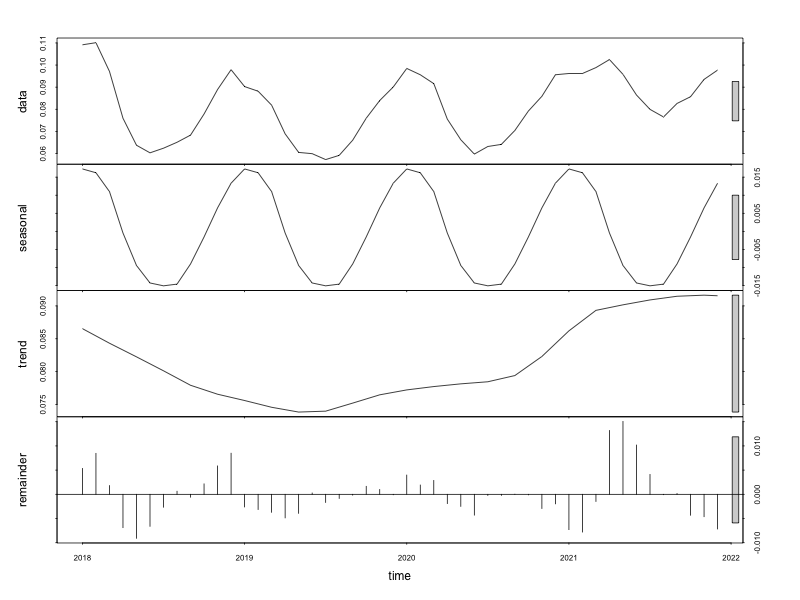
\includegraphics[width=0.75\linewidth]{stl_decomposition_plot.png}
        \caption{Trend for Unemployment}
        \label{fig:trend_unemp}
    \end{figure}
\end{frame}



\begin{frame}{Steps in the Analysis:}
    \textbf{Centered Log-Ratio Transformation:}
    \begin{itemize}
        \item A mathematical technique commonly used in \textbf{compositional data analysis} (CDA).
        \item Particularly useful for dealing with datasets where the components are proportions, percentages, or probabilities that sum to a constant (e.g., 1 or 100\%).

    \end{itemize}

\end{frame}

\begin{frame}{Steps in the Analysis:}
    \textbf{Centered Log-Ratio Transformation:}
For a compositional vector 
\[
\mathbf{x} = [x_1, x_2, \dots, x_D]
\]
where \( x_i > 0 \) and 
\[
\sum_{i=1}^{D} x_i = k \quad (\text{e.g., } k = 1 \text{ for proportions or } k = 100 \text{ for percentages}),
\]
the CLR transformation is given by:
\[
\text{CLR}(\mathbf{x}) = \left[ \log \left( \frac{x_1}{g(\mathbf{x})} \right), \log \left( \frac{x_2}{g(\mathbf{x})} \right), \dots, \log \left( \frac{x_D}{g(\mathbf{x})} \right) \right]
\]
where \( g(\mathbf{x}) \) is the geometric mean of the components:
\[
g(\mathbf{x}) = \left( \prod_{i=1}^{D} x_i \right)^{1/D}
\]

\end{frame}

\begin{frame}{Steps in the Analysis:}
    \textbf{Centered Log-Ratio Transformation:}

    \begin{itemize}
        \item Compositional data have a \textbf{constant-sum constraint}, which can create spurious correlations. The \textbf{CLR transformation removes this issue} by transforming the data into a log-ratio scale.
        \item The CLR-transformed values indicate the \textbf{log-relative contributions} of each component \textbf{compared to the geometric mean}.
        \item Removes the closure problem and \textbf{allows for clustering methods}. 
    \end{itemize}

\end{frame}

\begin{frame}{Steps in the Analysis:}
    \textbf{Advantages of Clustering Methods:}

    \begin{itemize}
        \item Instead of isolating variables (like subgroups), \textbf{considers all CLR variables simultaneously}, capturing \textbf{interrelationships} across categories.
        \item Can uncover \textbf{patterns} or \textbf{groupings} across compositional features.
        \item Can reveal \textbf{temporal shifts} in proportions when applied to \textbf{time-series data}.

    \end{itemize}

\end{frame}

\begin{frame}{Steps in the Analysis:}
    \textbf{Two Types of Clustering Methods:}
    \begin{table}[]
    \centering
    \resizebox{\linewidth}{!}{%
    \begin{tabular}{|l|l|l|}
    \hline
    \textbf{Feature}       & \textbf{Hierarchical Clustering}          & \textbf{K-Means Clustering}         \\ \hline
    \textbf{Approach}      & Builds a hierarchy of clusters.          & Iteratively partitions data into $k$ clusters. \\ \hline
    \textbf{Input Requirement}         & Distance matrix or raw data.             & Raw data and number of clusters ($k$). \\ \hline
    \textbf{Output}        & Dendrogram, clusters at chosen level.    & Final cluster assignments.           \\ \hline
    \textbf{Sensitivity}   & Stable across seeds; sensitive to linkage method. & Sensitive to seed choice; faster but less stable. \\ \hline
    \textbf{Use Case} & Suitable for smaller datasets with unknown cluster numbers. &	Ideal for large datasets with a known number of clusters. \\ \hline
    \end{tabular}%
    }
    \caption{Comparison of Clustering Methods}
    \end{table}
\end{frame}







\section{Findings}

\begin{frame}
    \frametitle{Findings}
    \begin{figure}
        \centering
        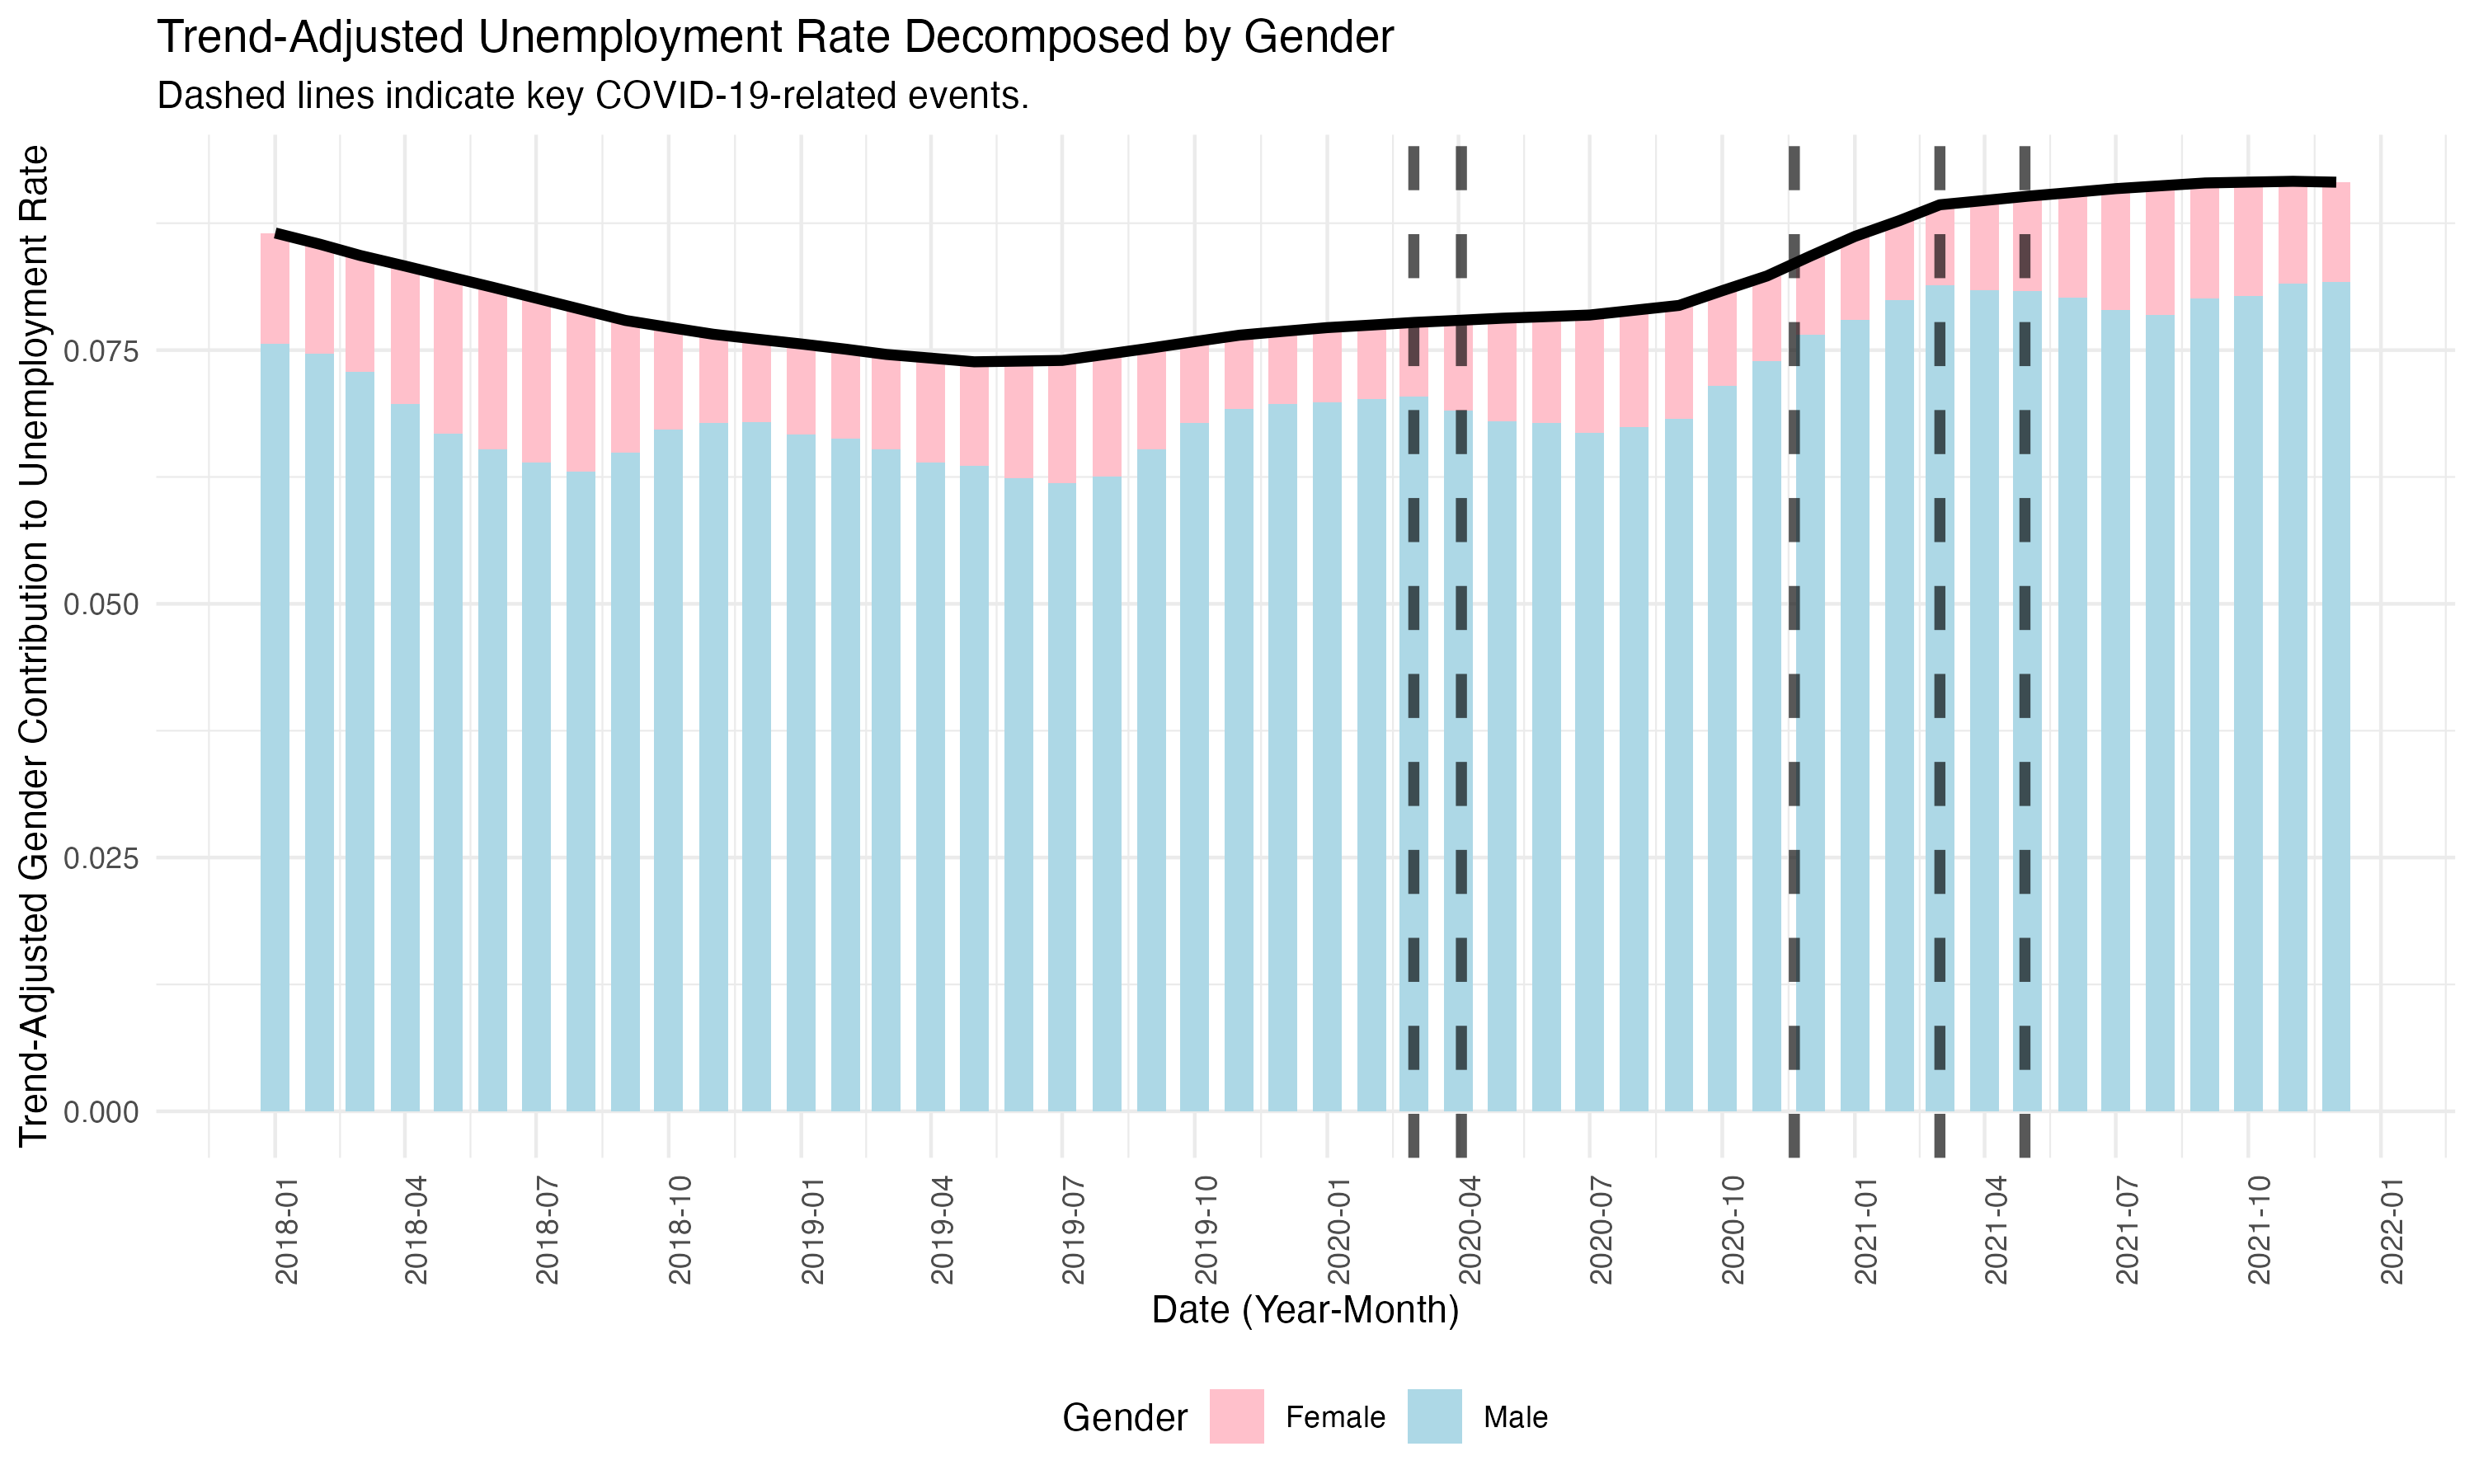
\includegraphics[width=0.75\linewidth]{gender_adjusted_plot.png}
        \caption{Trend Adjusted Unemployment - Gender Decomposition}
        \label{fig:trend_adj_gender}
    \end{figure}
\end{frame}

\begin{frame}
    \frametitle{Findings}
    \begin{figure}
        \centering
        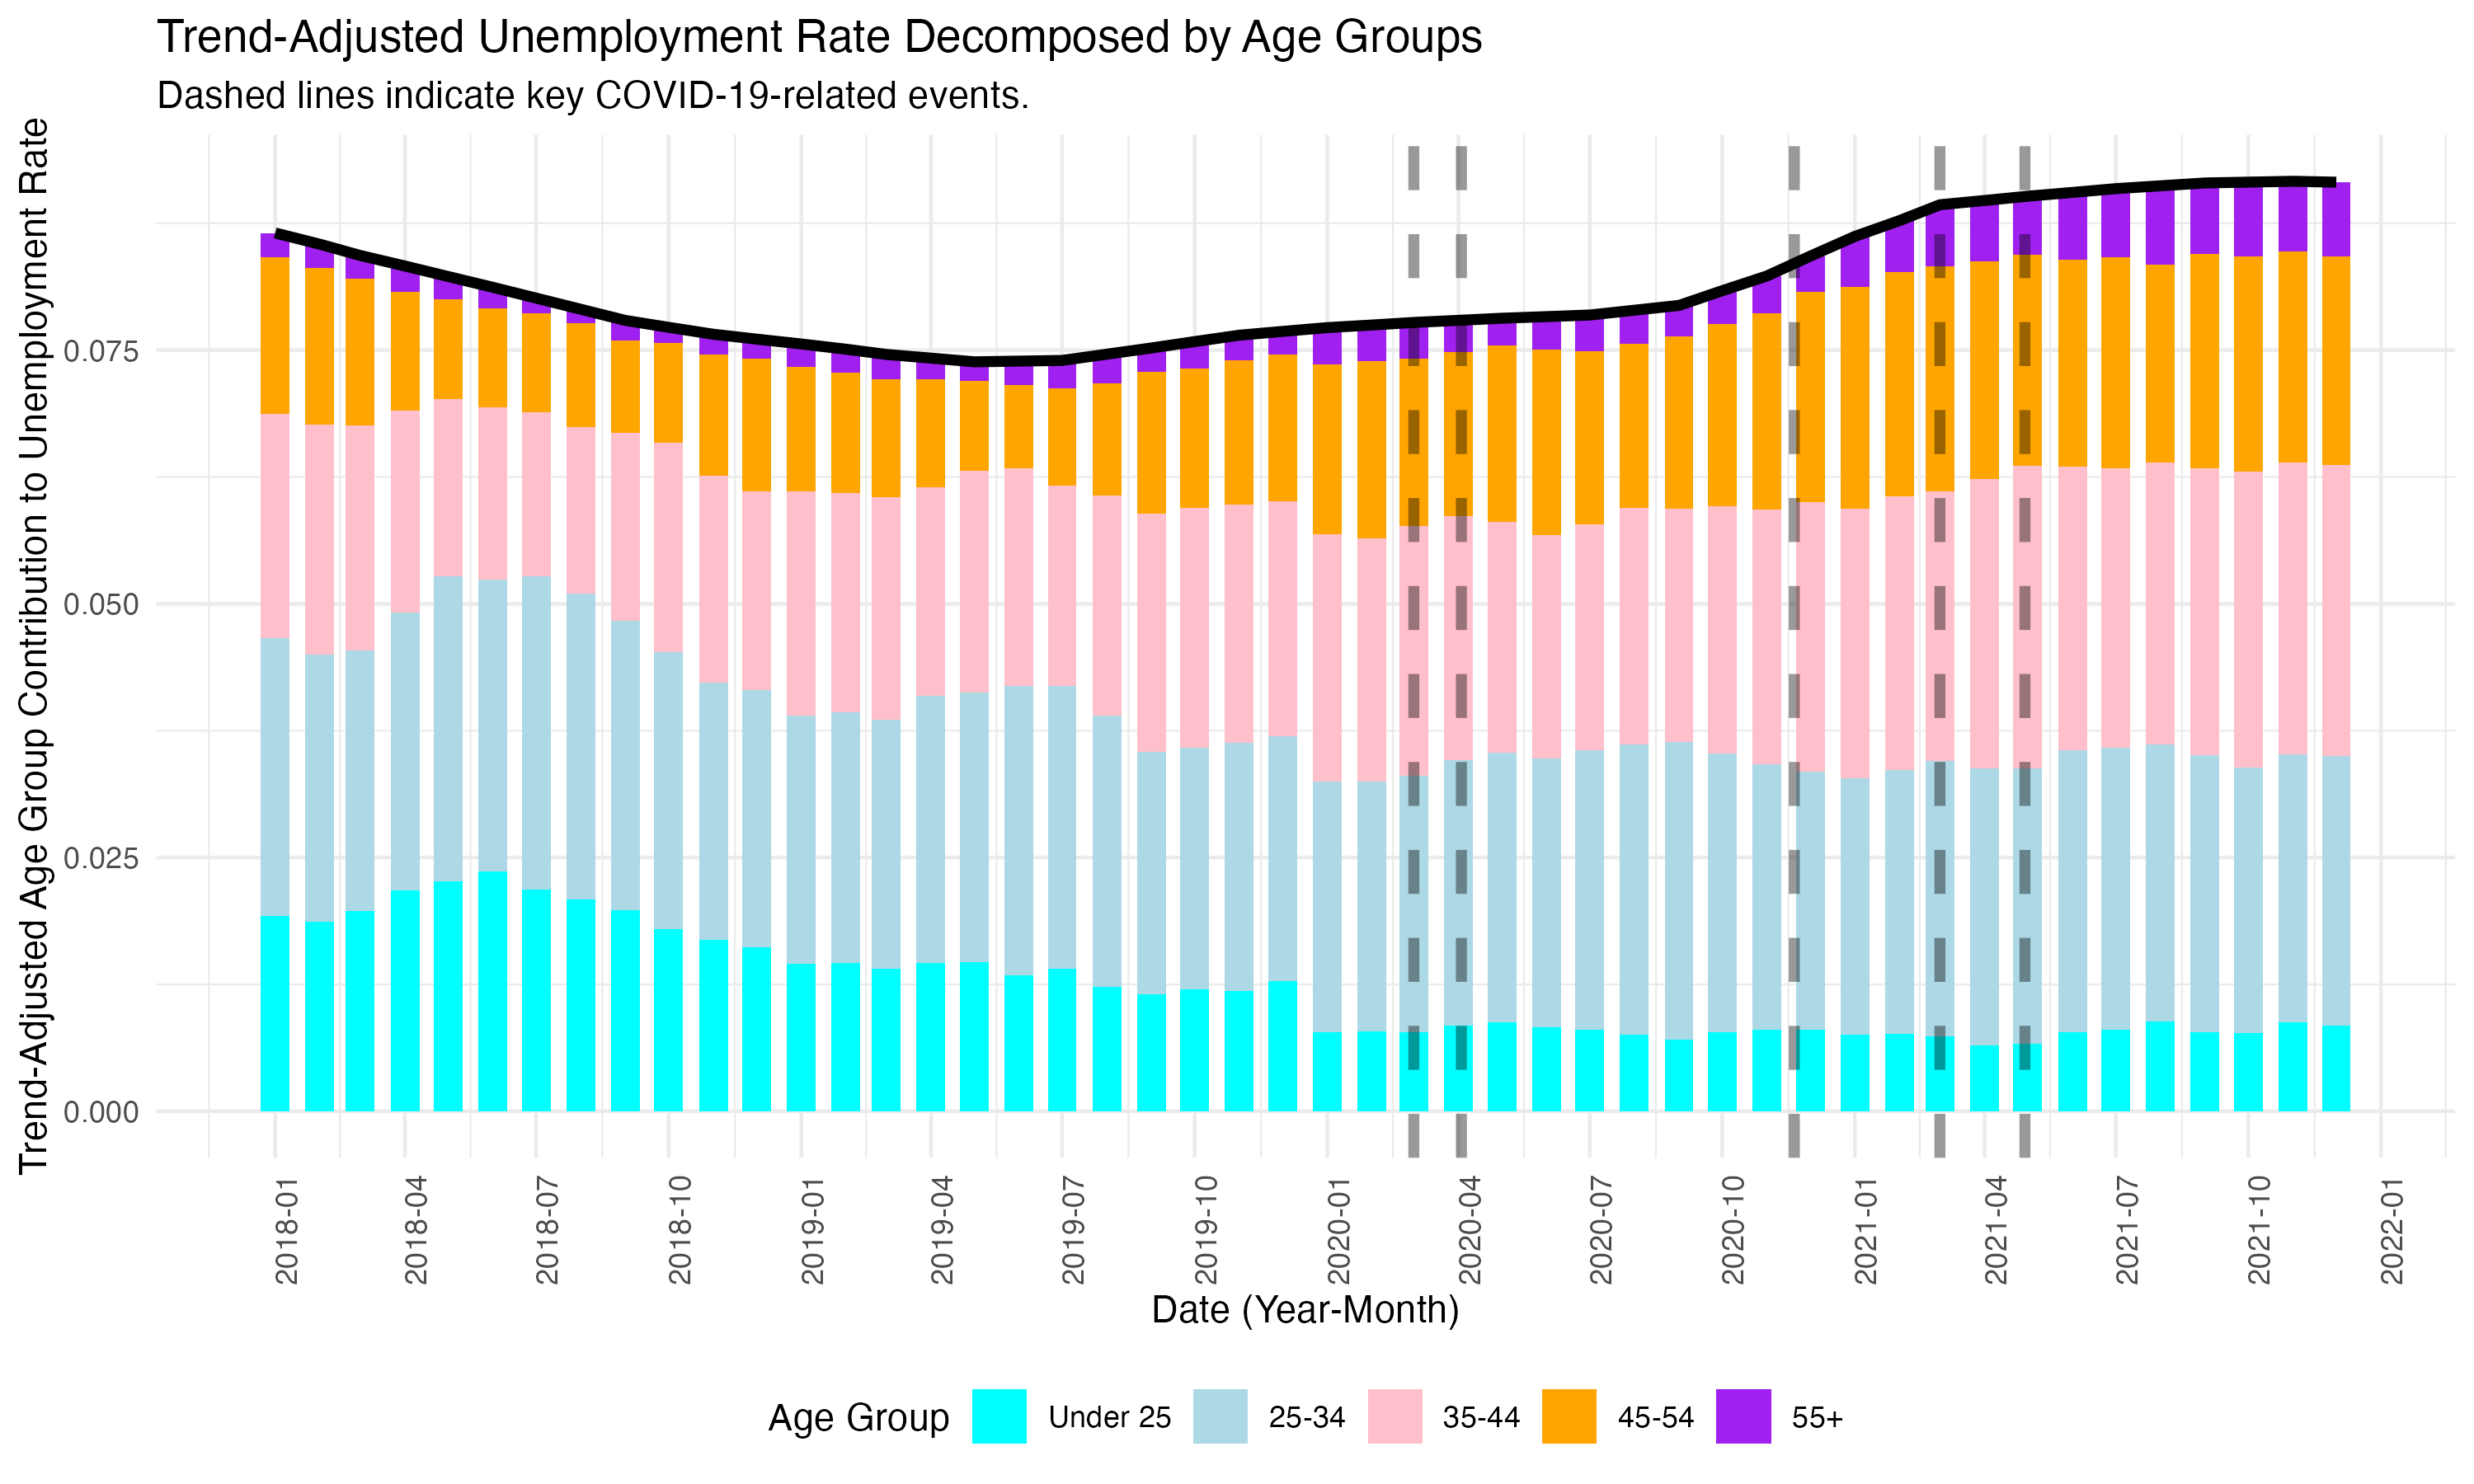
\includegraphics[width=0.75\linewidth]{age_adjusted_plot.png}
        \caption{Trend Adjusted Unemployment - Age Groups}
        \label{fig:trend_adj_age}
    \end{figure}
\end{frame}

\begin{frame}
    \frametitle{Findings}
    \begin{figure}
            \centering
            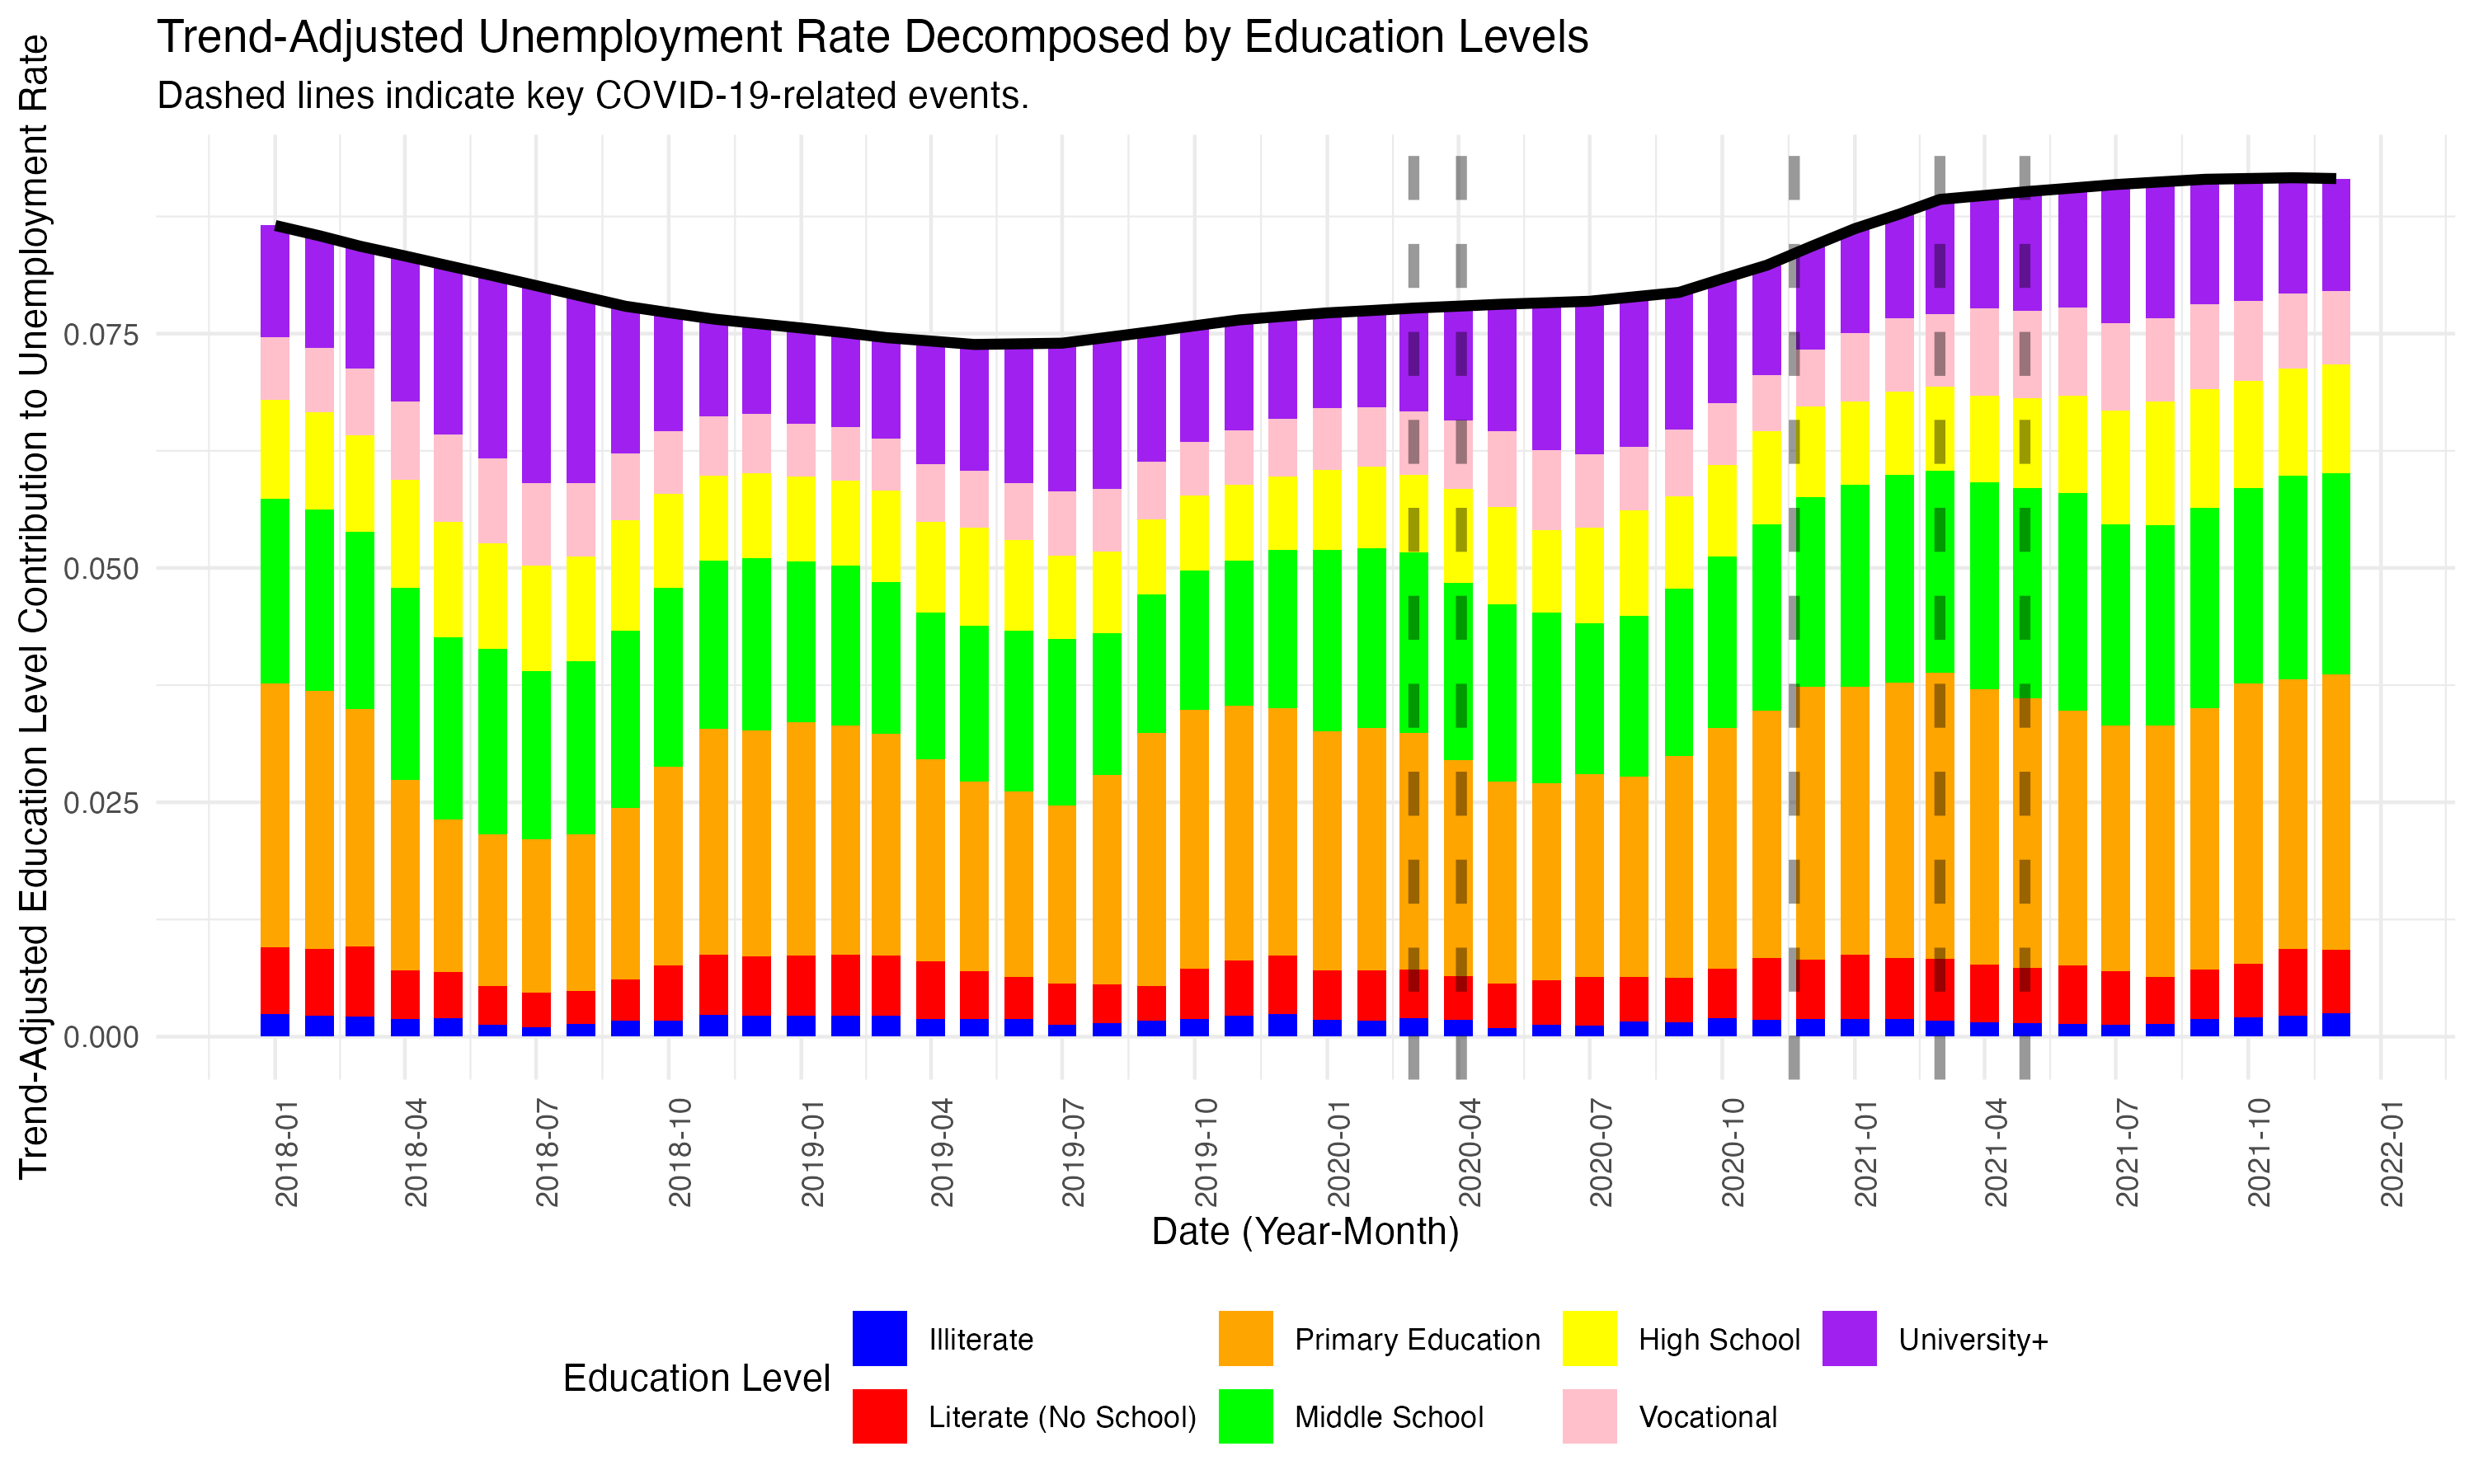
\includegraphics[width=0.75\linewidth]{education_adjusted_plot.png}
            \caption{Trend Adjusted Unemployment - Education Levels}
            \label{fig:trend_adj_educ}
        \end{figure}
\end{frame}

\begin{frame}
    \frametitle{Findings}
    \begin{figure}
        \centering
        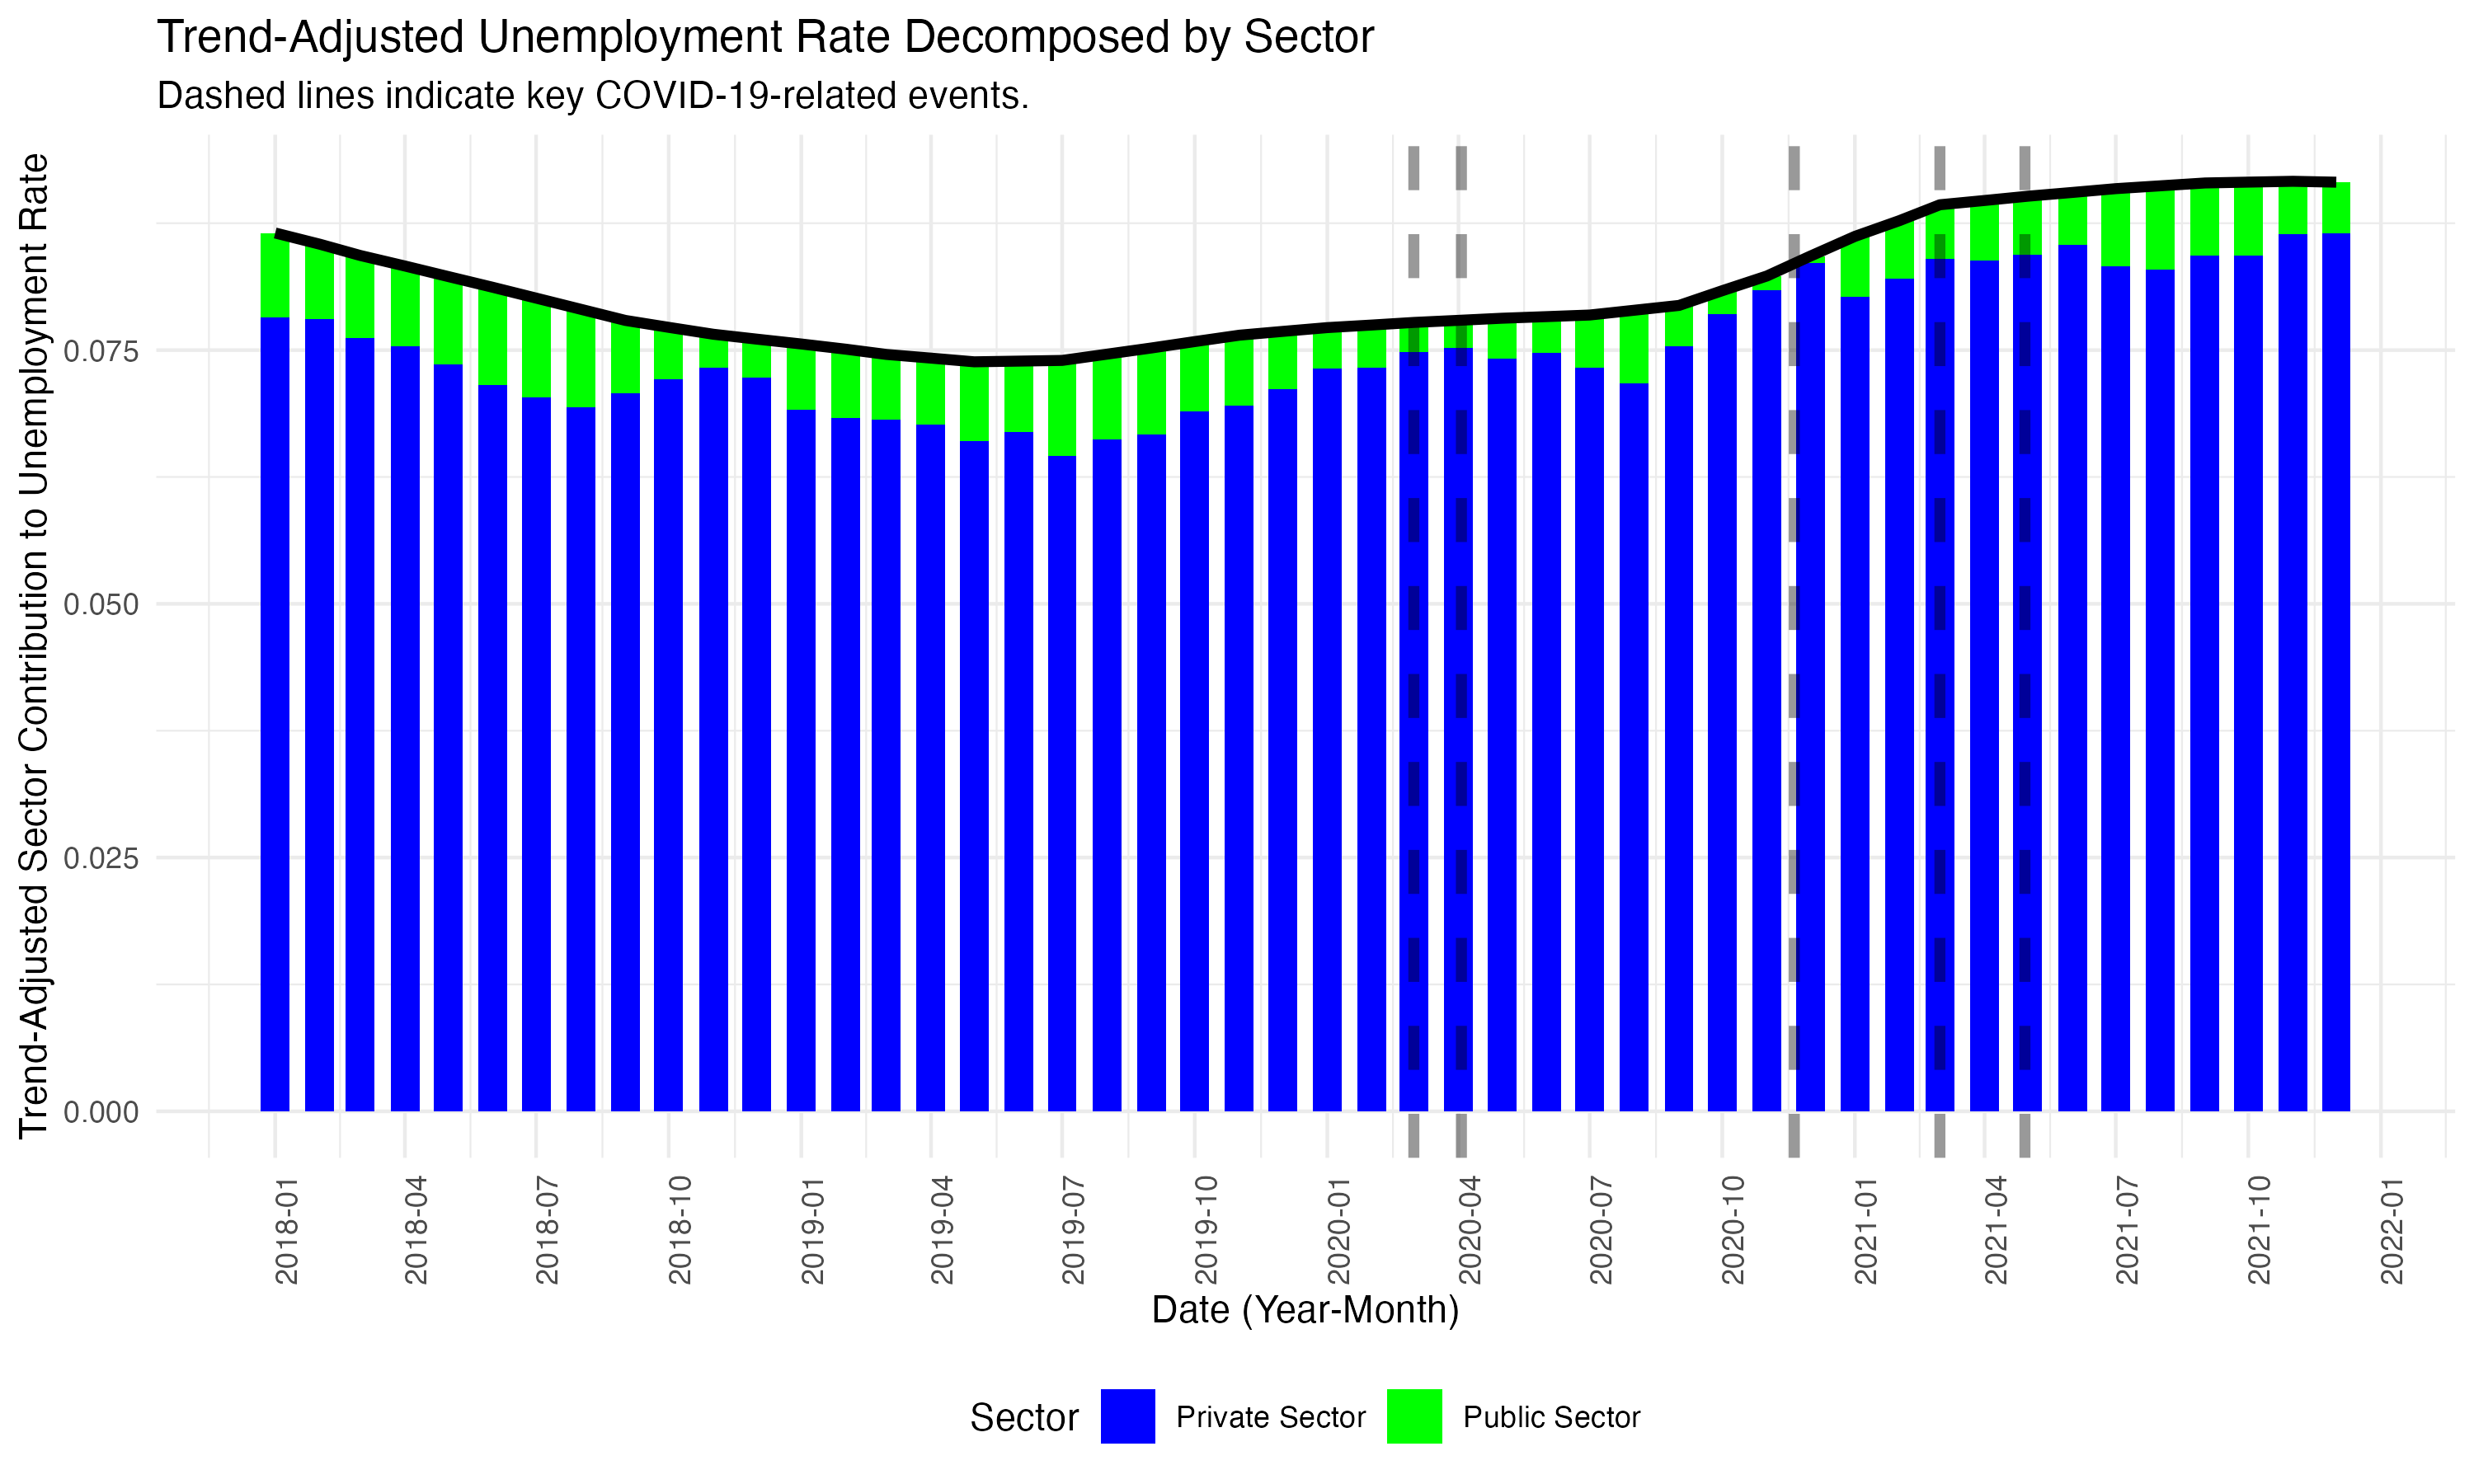
\includegraphics[width=0.75\linewidth]{sector_adjusted_plot.png}
        \caption{Trend Adjusted Unemployment - Establishment Decomposition}
        \label{fig:trend_adj_pubpriv}
    \end{figure}
\end{frame}

\begin{frame}
    \frametitle{Findings}
    \begin{figure}
        \centering
        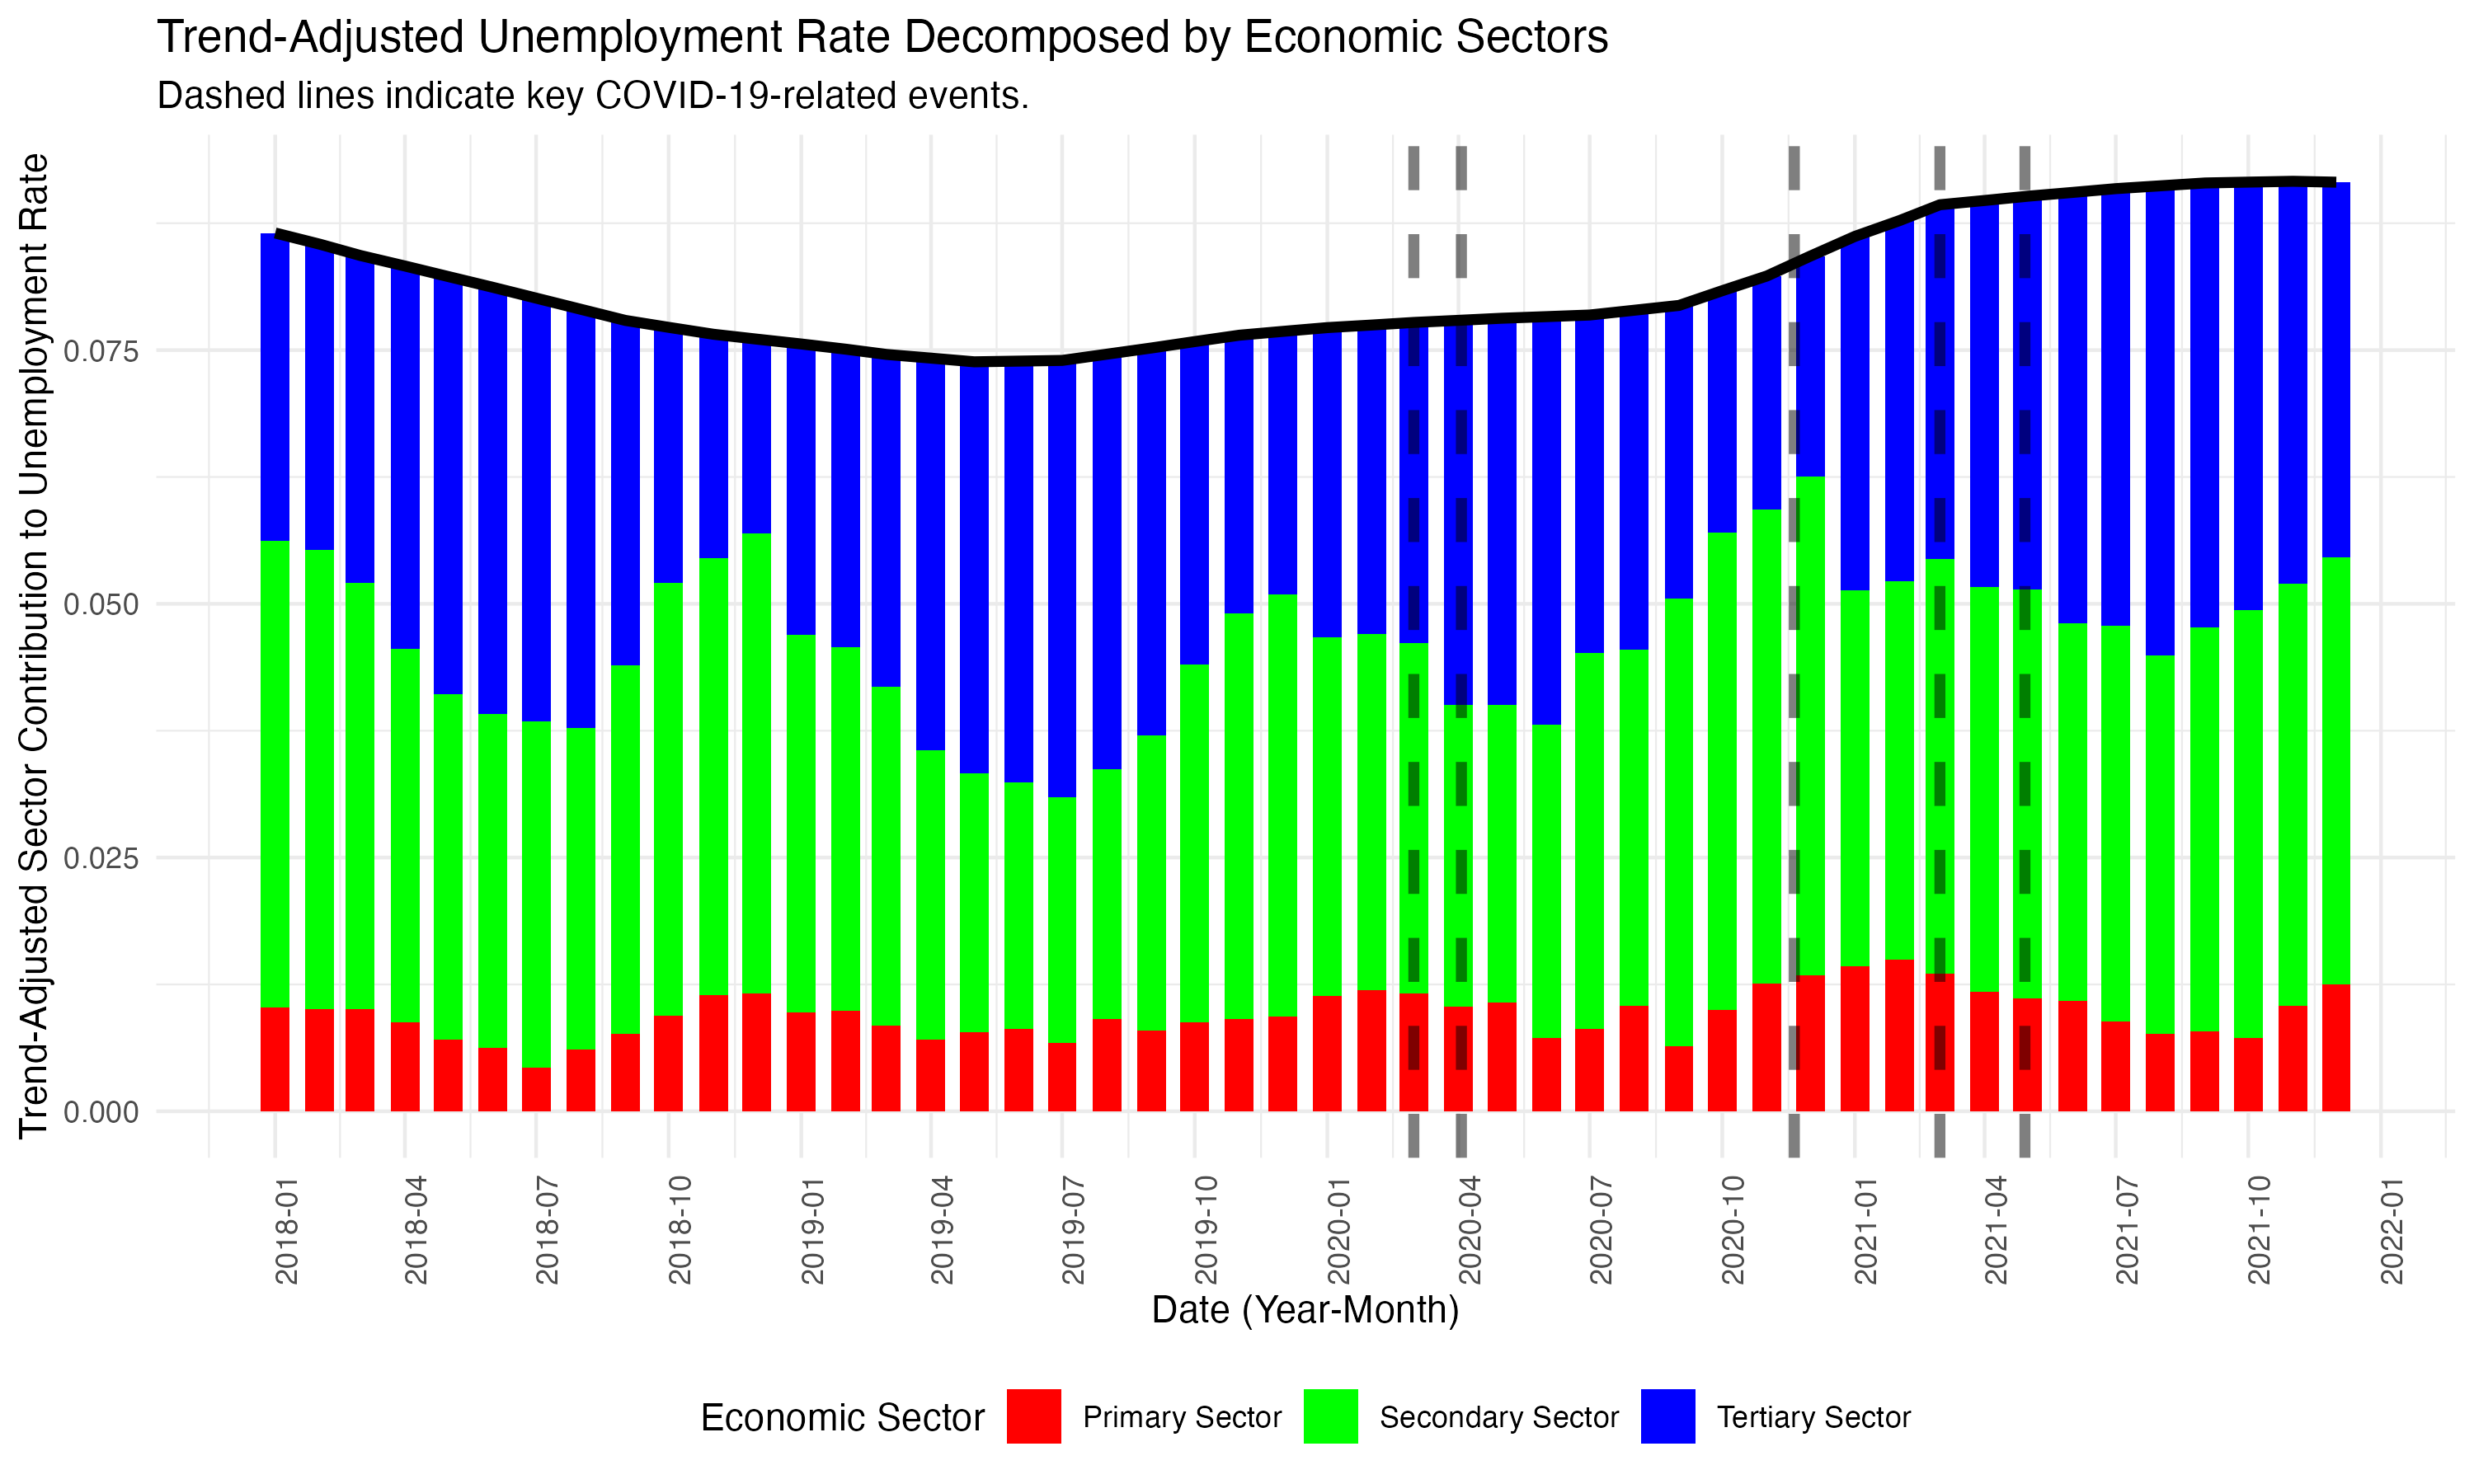
\includegraphics[width=0.75\linewidth]{trend_adjusted_plot.png}
        \caption{Trend Adjusted Unemployment - Sectoral Decomposition}
        \label{fig:trend_adj_threesectors}
    \end{figure}
\end{frame}

\begin{frame}
    \frametitle{Findings}
    \begin{figure}
        \centering
        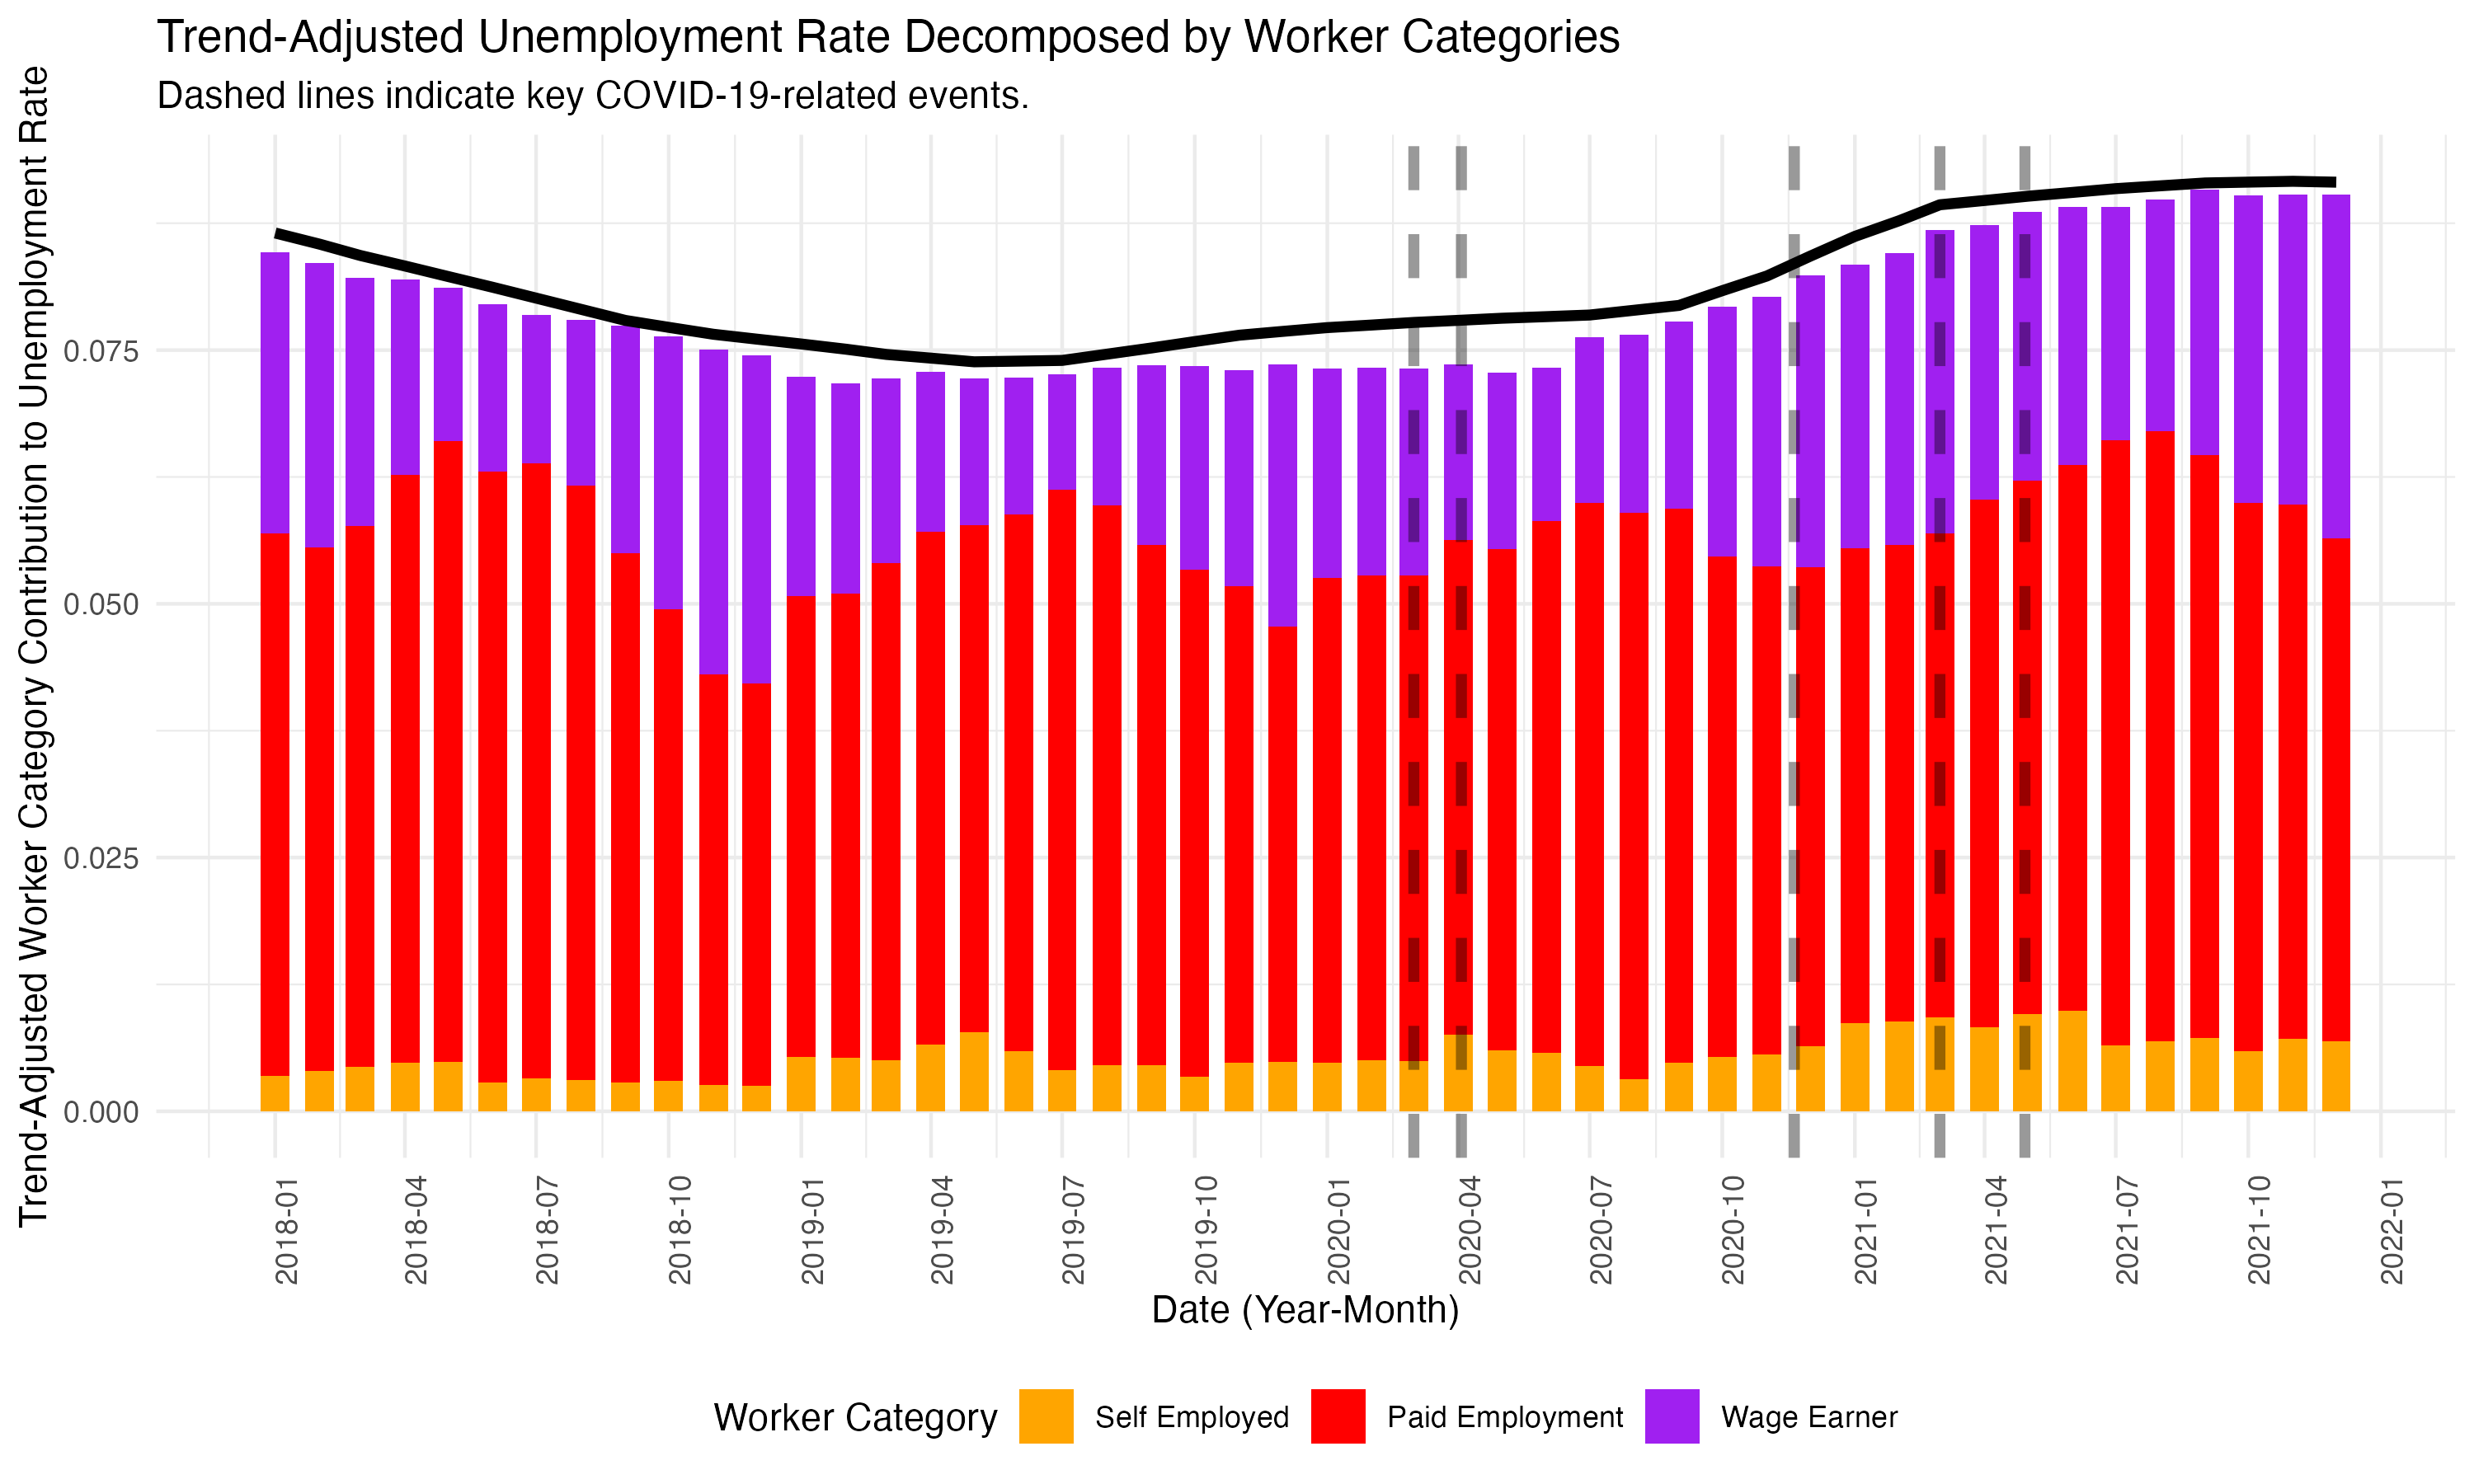
\includegraphics[width=0.75\linewidth]{worker_adjusted_plot.png}
        \caption{Trend Adjusted Unemployment - Employment Types}
        \label{fig:trend_adj_employment}
    \end{figure}
\end{frame}

\begin{frame}
    \frametitle{Findings}
    \begin{figure}
        \centering
        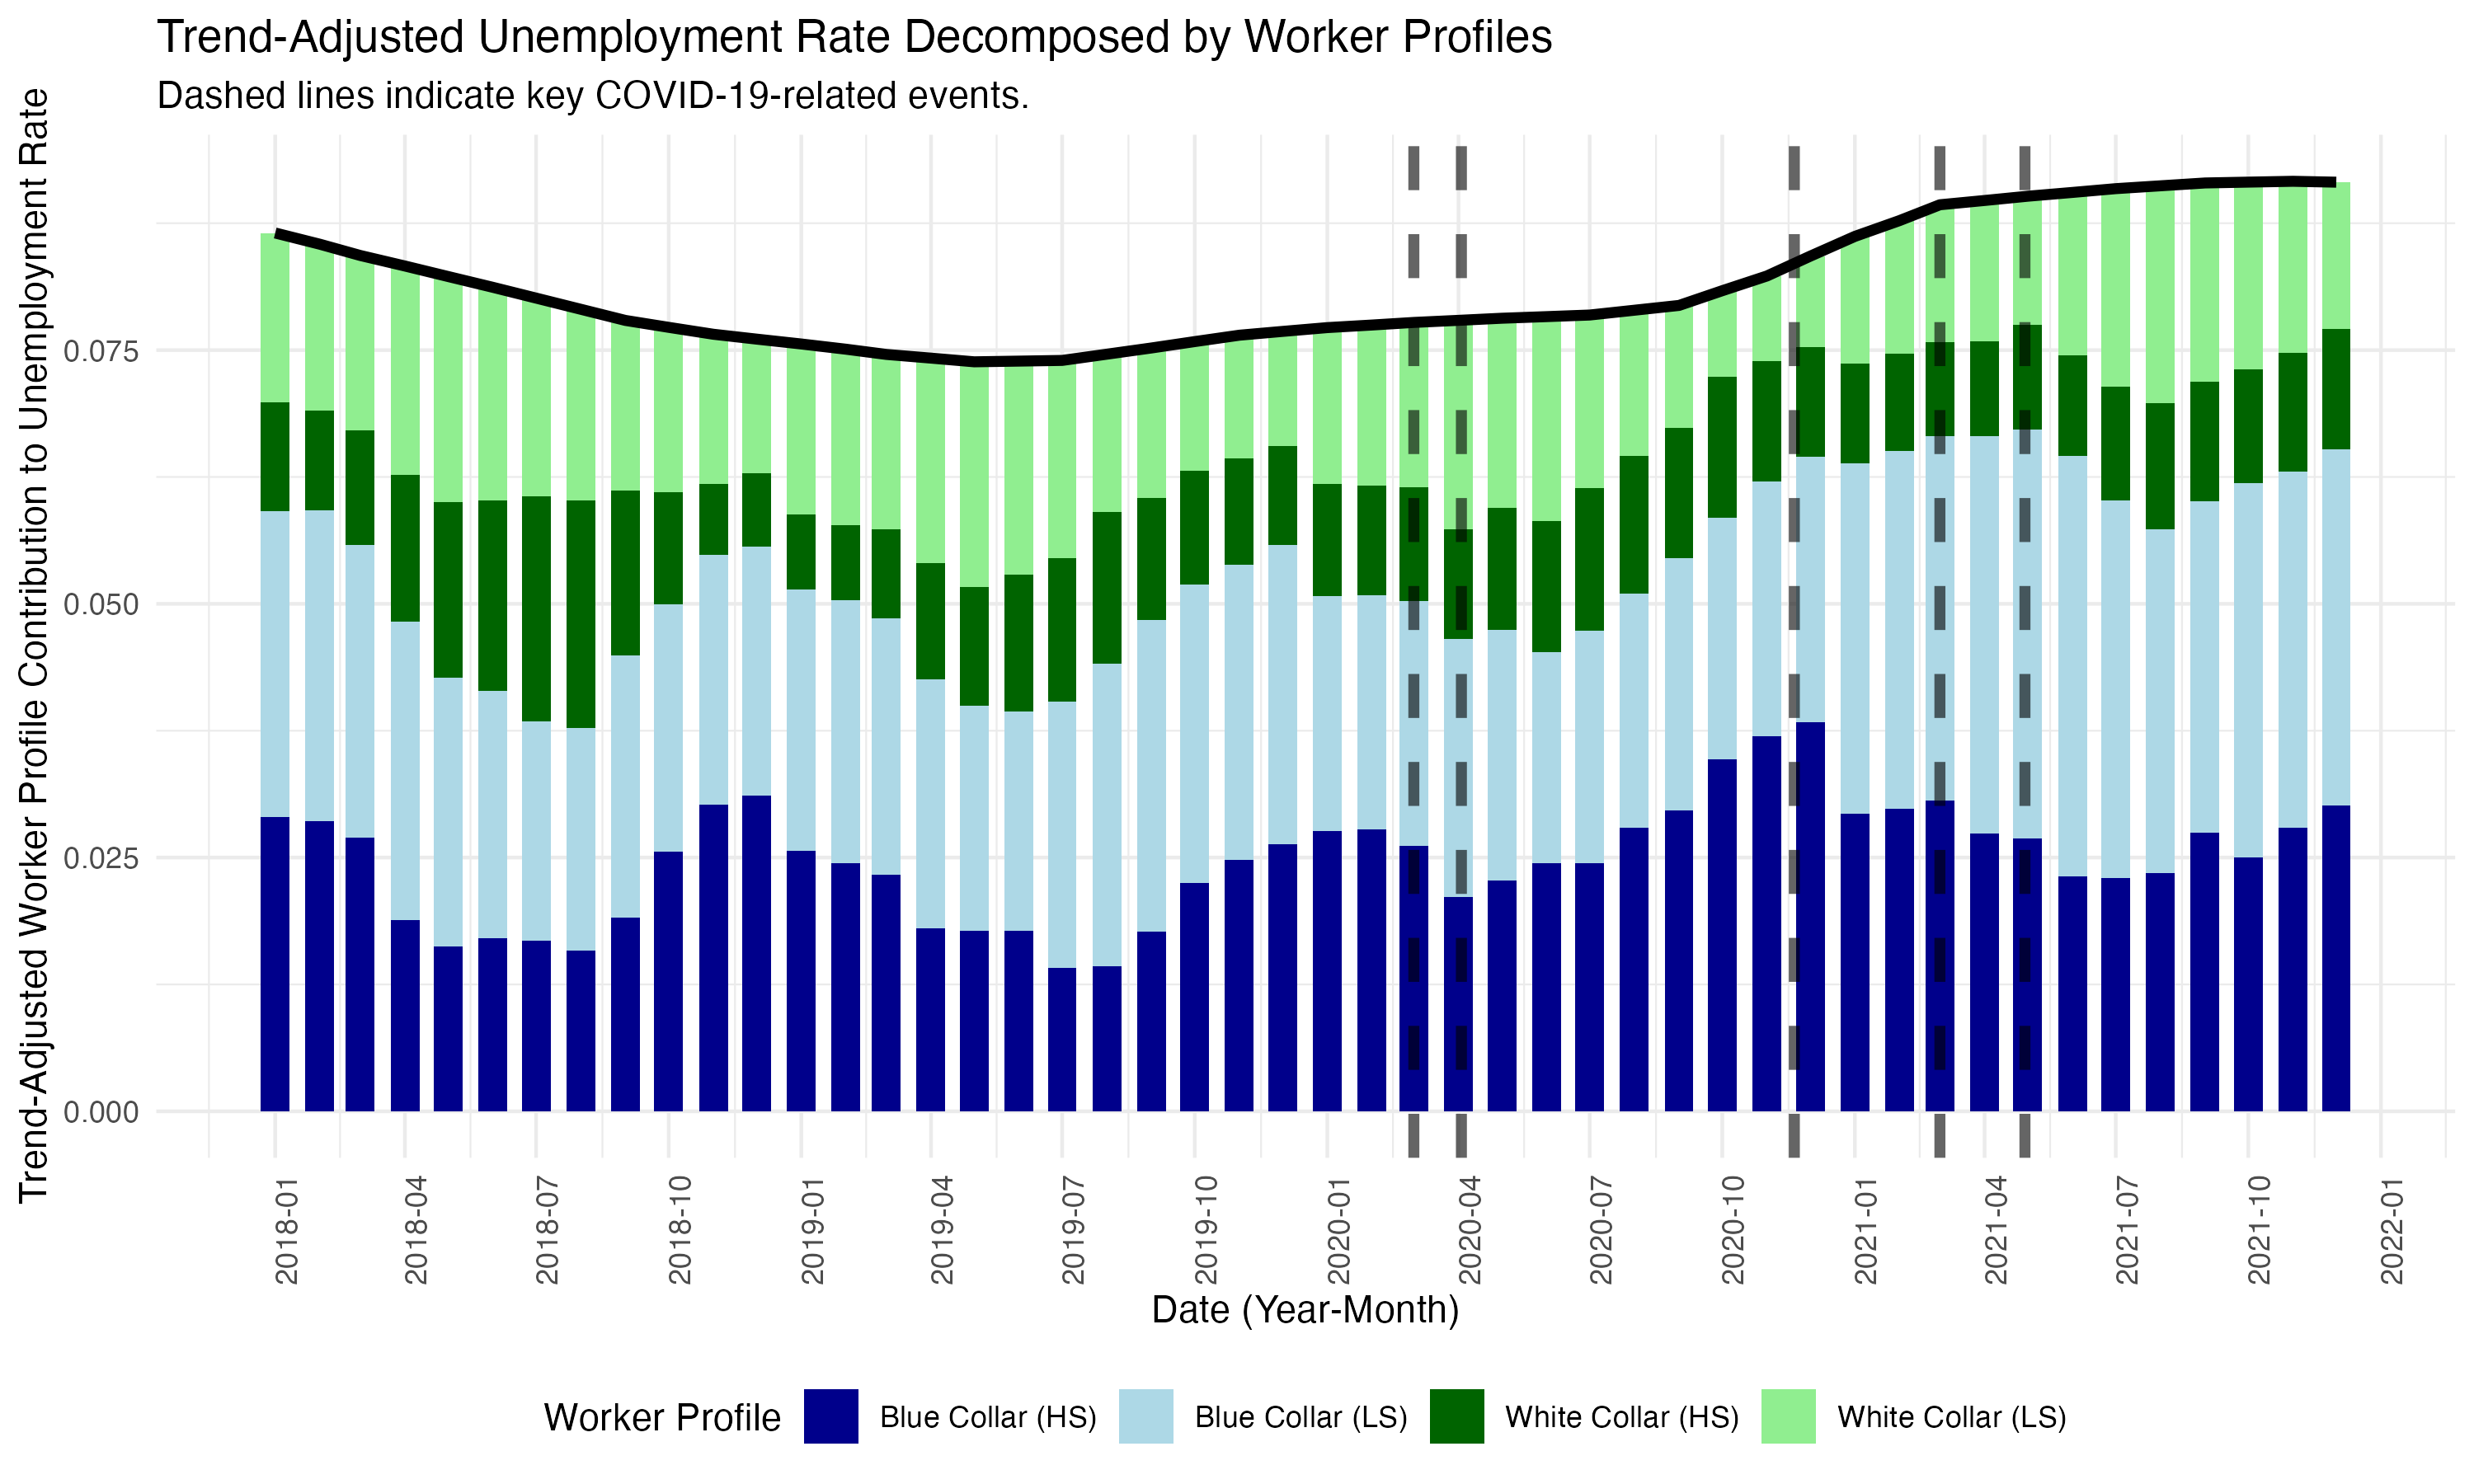
\includegraphics[width=0.75\linewidth]{trend_adj_worker_prof.png}
        \caption{Trend Adjusted Unemployment - Worker Profiles}
        \label{fig:trend_adj_workprof}
    \end{figure}
\end{frame}

\begin{frame}
    \frametitle{Findings}
    \begin{figure}
        \centering
        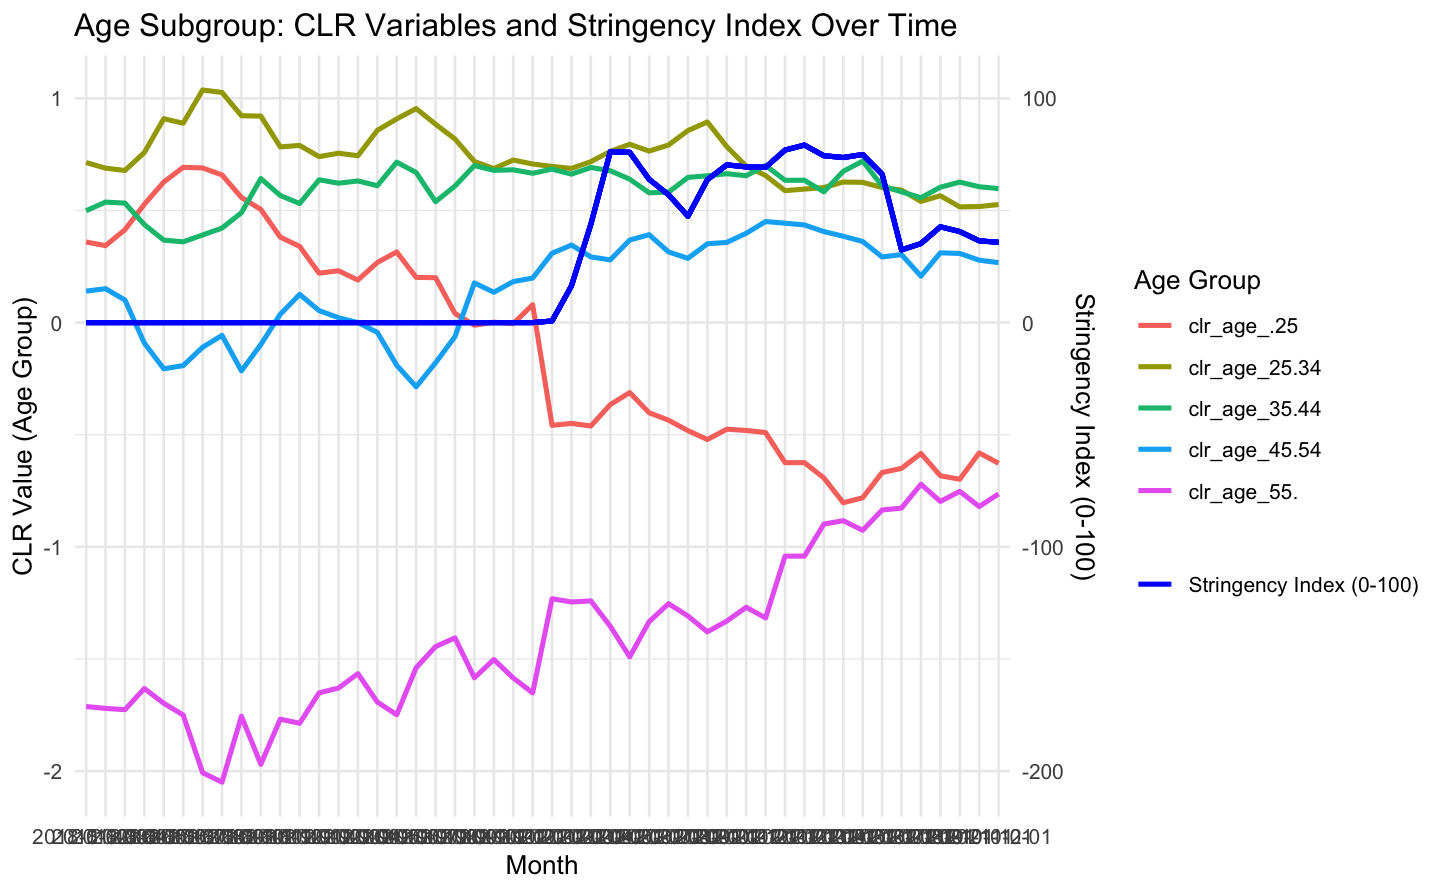
\includegraphics[width=0.75\linewidth]{clr_str_age.png}
        \caption{CLR-Transformed Age Groups and Stringency Index}
        \label{fig:clr_str_age}
    \end{figure}
\end{frame}

\begin{frame}
    \frametitle{Findings}
    \begin{figure}
        \centering
        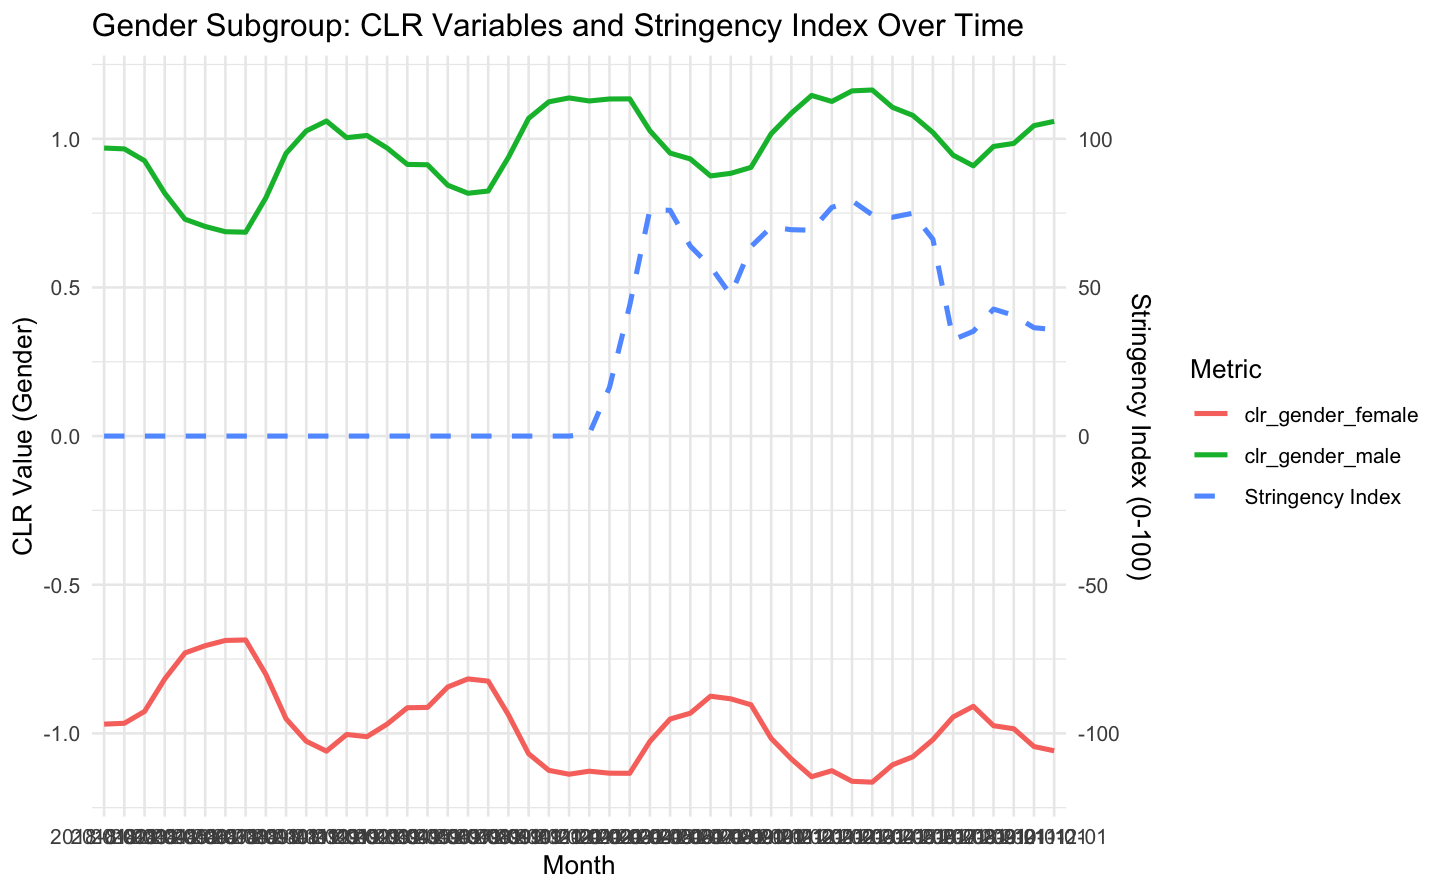
\includegraphics[width=0.75\linewidth]{clr_str_gender.png}
        \caption{CLR-Transformed Genders and Stringency Index}
        \label{fig:clr_str_gender}
    \end{figure}
\end{frame}


\begin{frame}
    \frametitle{Findings}
    \begin{figure}
        \centering
        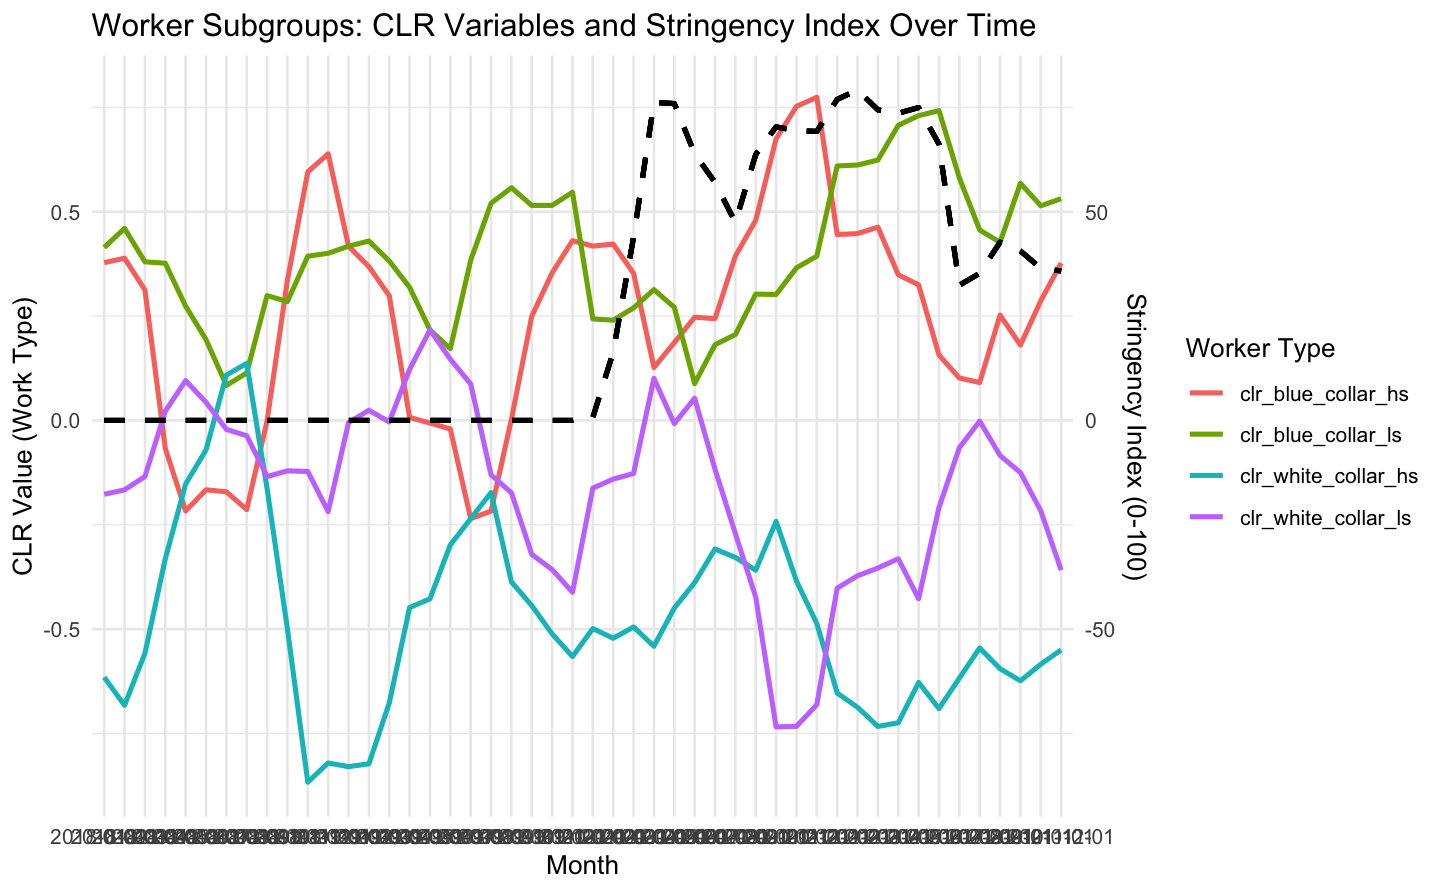
\includegraphics[width=0.75\linewidth]{clr_str_wp.png}
        \caption{CLR-Transformed Worker Profiles and Stringency Index}
        \label{fig:clr_str_wp}
    \end{figure}
\end{frame}


\begin{frame}
    \frametitle{Findings}
    \begin{figure}
        \centering
        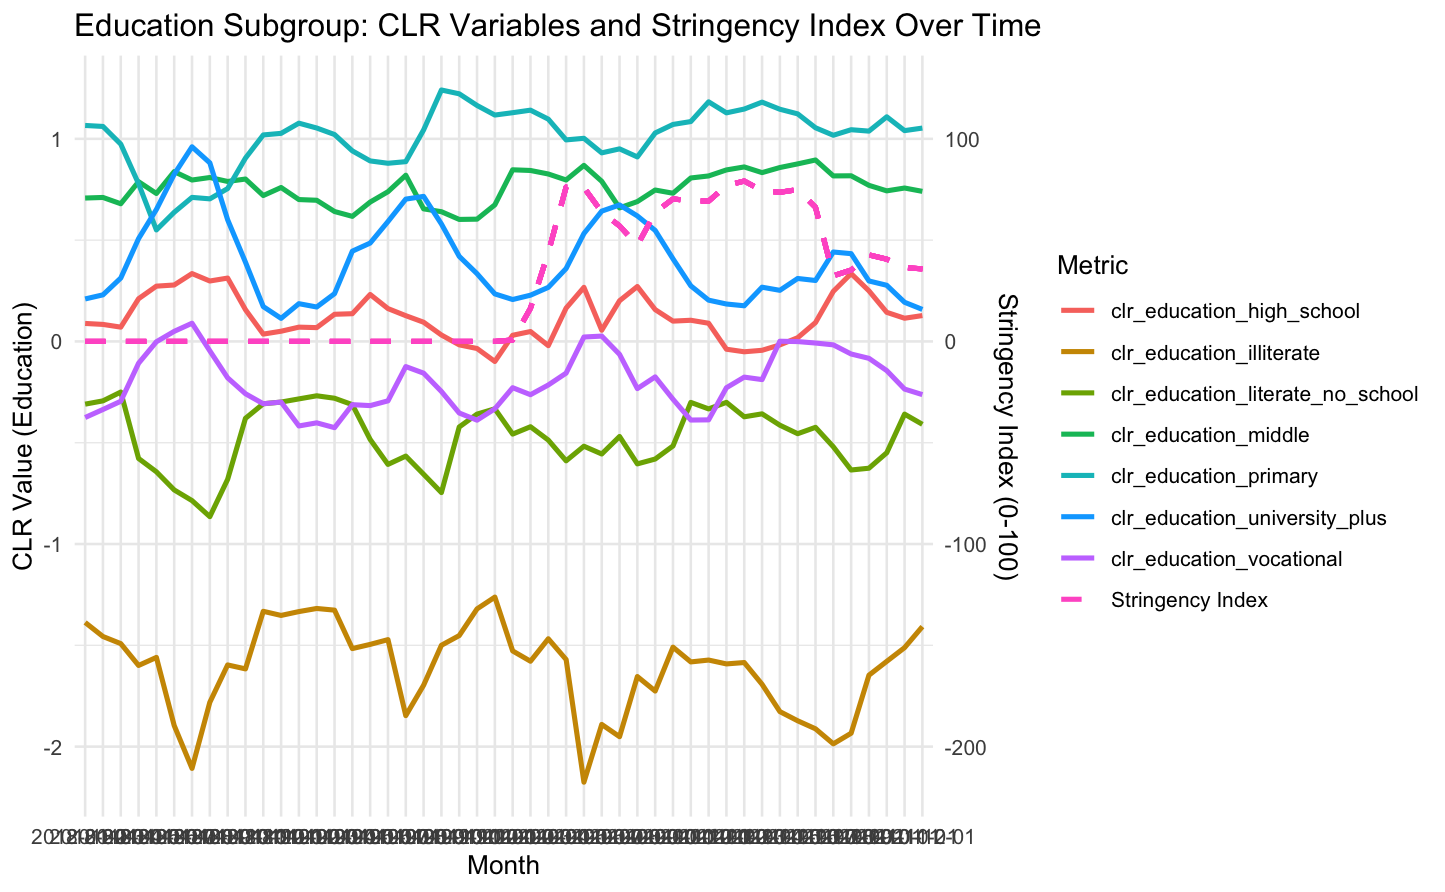
\includegraphics[width=0.75\linewidth]{clr_str_educ.png}
        \caption{CLR-Transformed Education Groups and Stringency Index}
        \label{fig:enter-label}
    \end{figure}
\end{frame}

\begin{frame}
    \frametitle{Findings}
    \begin{figure}
        \centering
        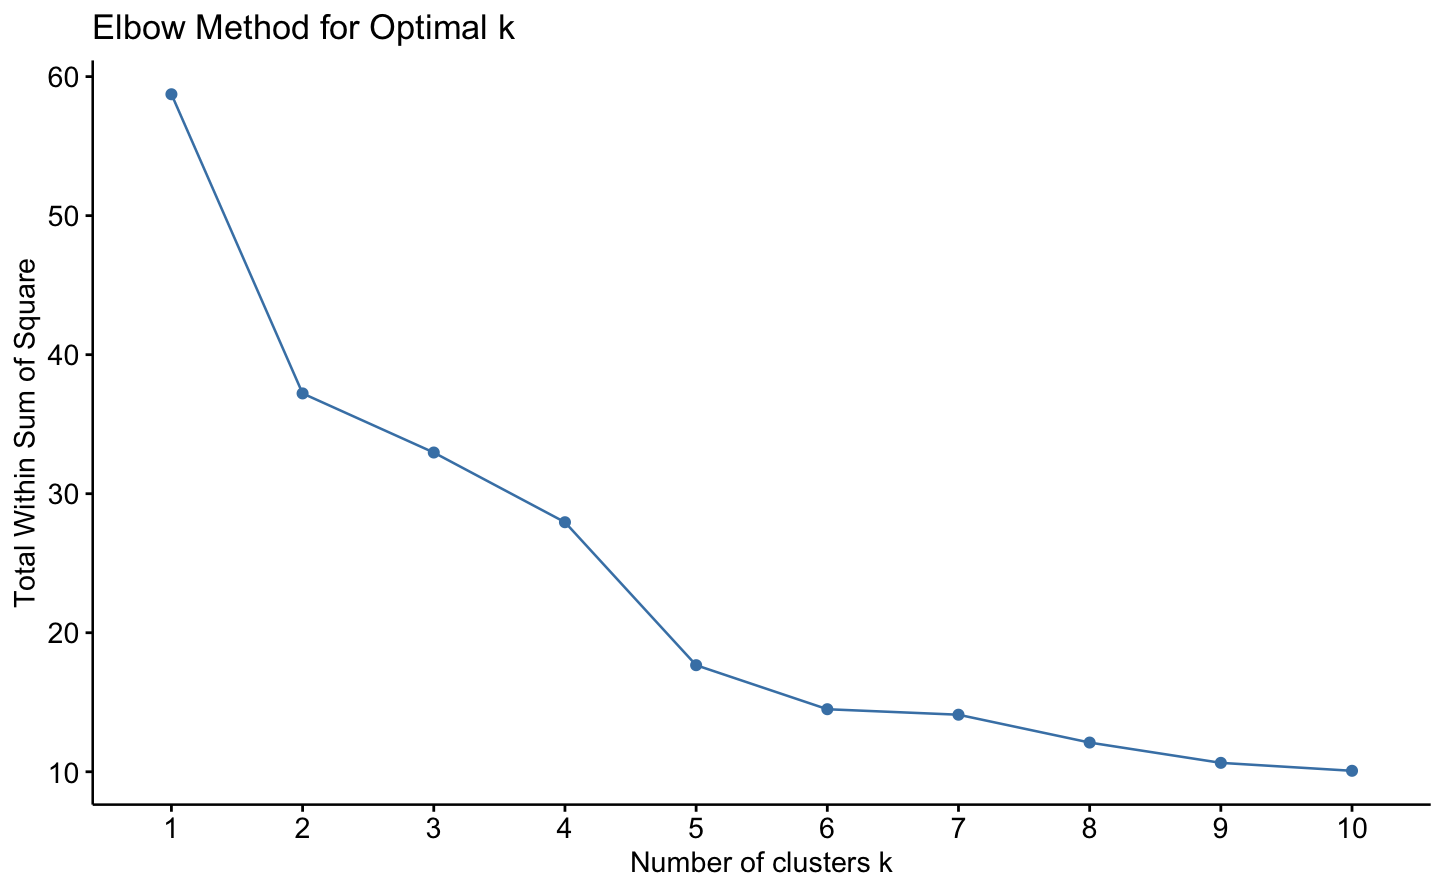
\includegraphics[width=0.75\linewidth]{elbow method.png}
        \caption{Elbow Method for k-mean Clustering Method}
        \label{fig:elbow method}
    \end{figure}
\end{frame}

\begin{frame}
    \frametitle{Findings}
    \begin{figure}
        \centering
        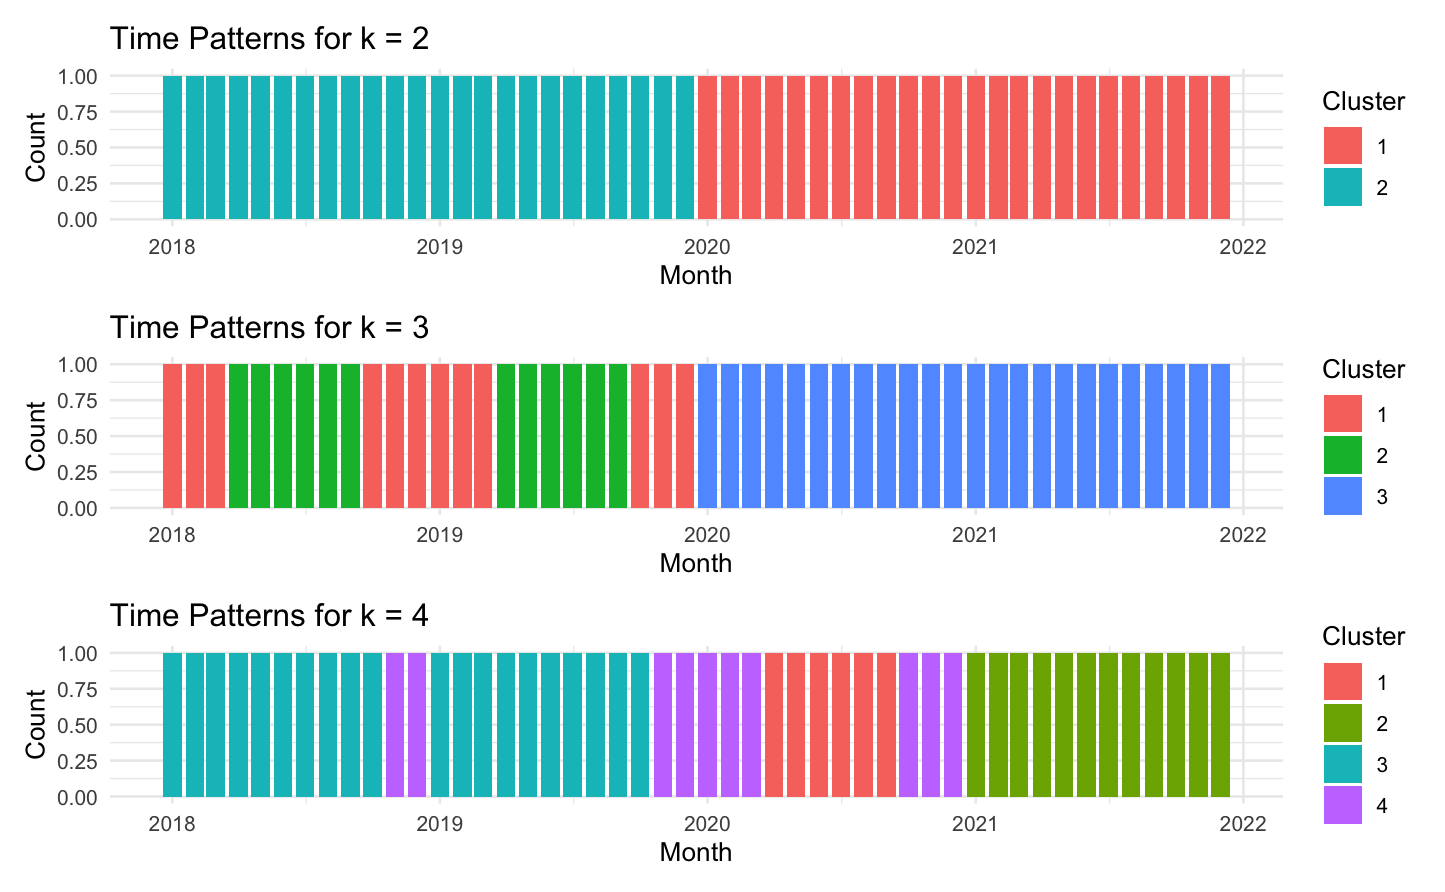
\includegraphics[width=0.75\linewidth]{clr_kmean_123.png}
        \caption{Different Clusters of k-mean for seed: 123}
        \label{fig:clr_kmean_123}
    \end{figure}
\end{frame}

\begin{frame}
    \begin{figure}
        \centering
        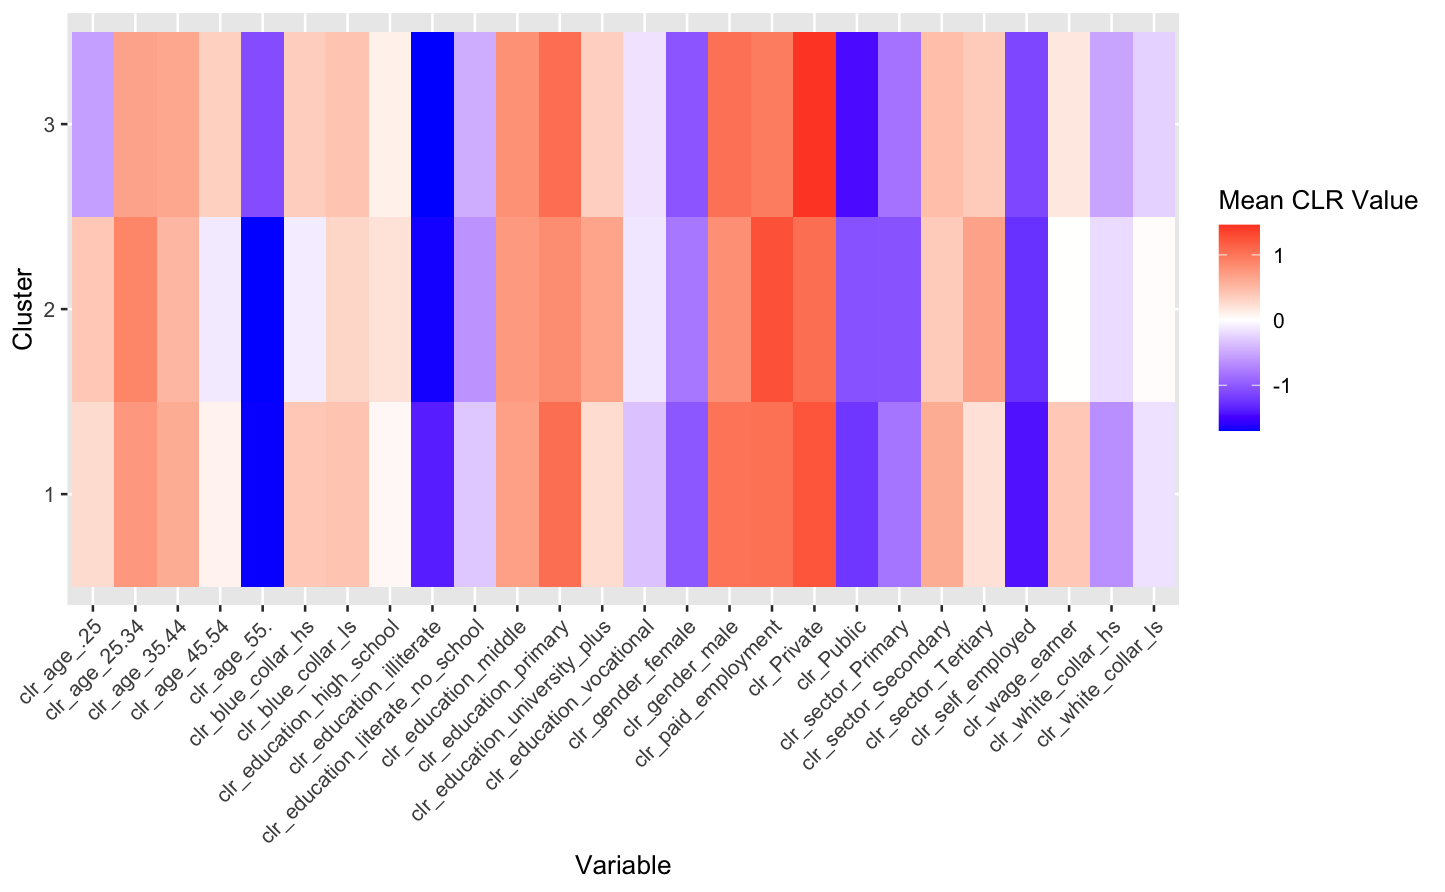
\includegraphics[width=0.75\linewidth]{clr_kmean_heatmap.png}
        \caption{Heatmap for k=3}
        \label{fig:clr_kmean_heatmap}
    \end{figure}
\end{frame}

\begin{frame}
    \begin{figure}
        \centering
        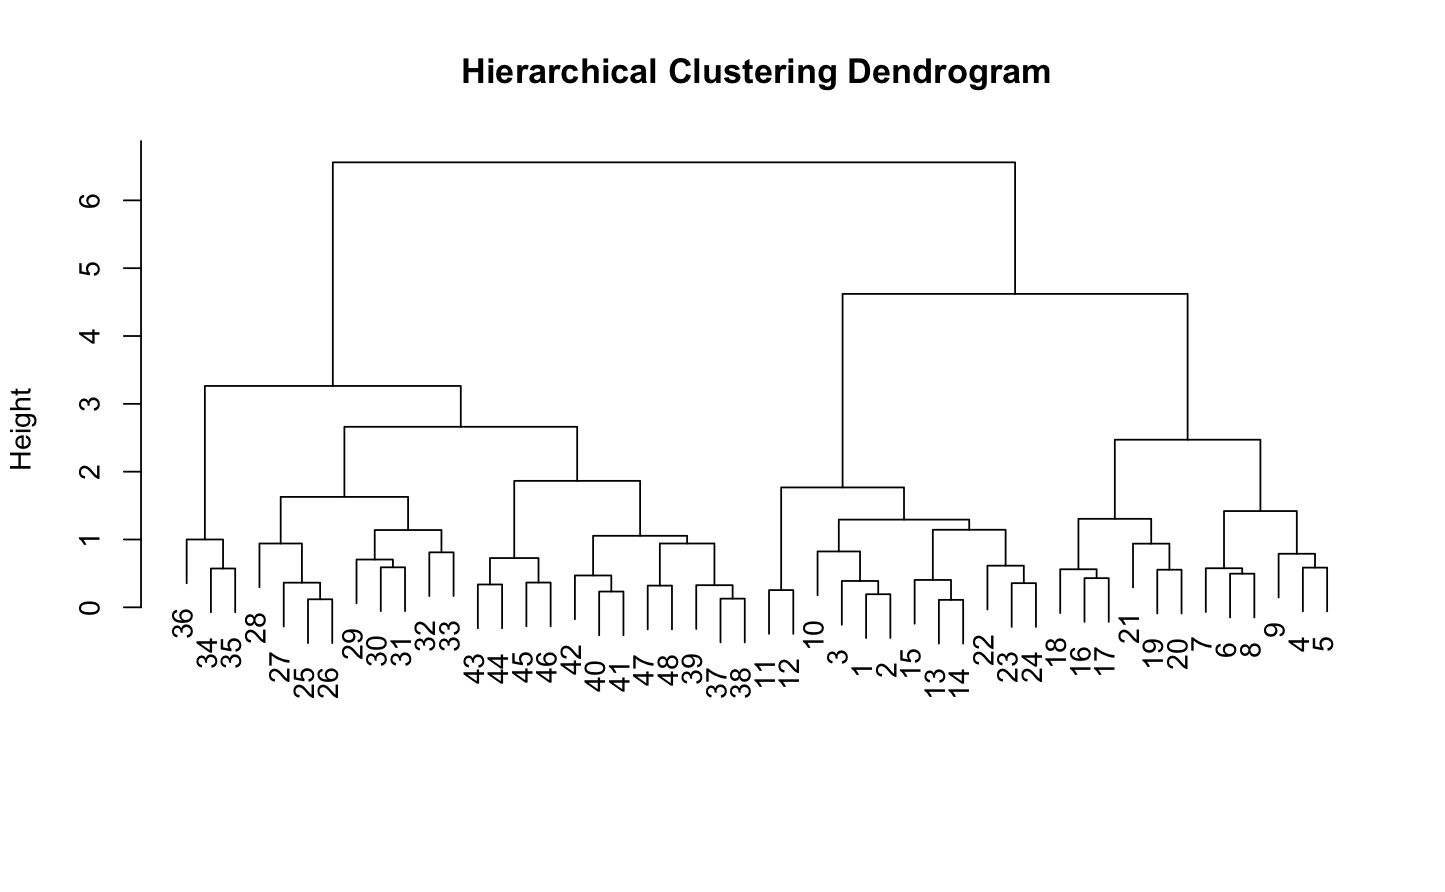
\includegraphics[width=0.75\linewidth]{clr_hier_dendo.png}
        \caption{Dendogram for Hiearchical Clustering Method}
        \label{fig:clr_hier_dendo}
    \end{figure}
\end{frame}

\begin{frame}
    \begin{figure}
        \centering
        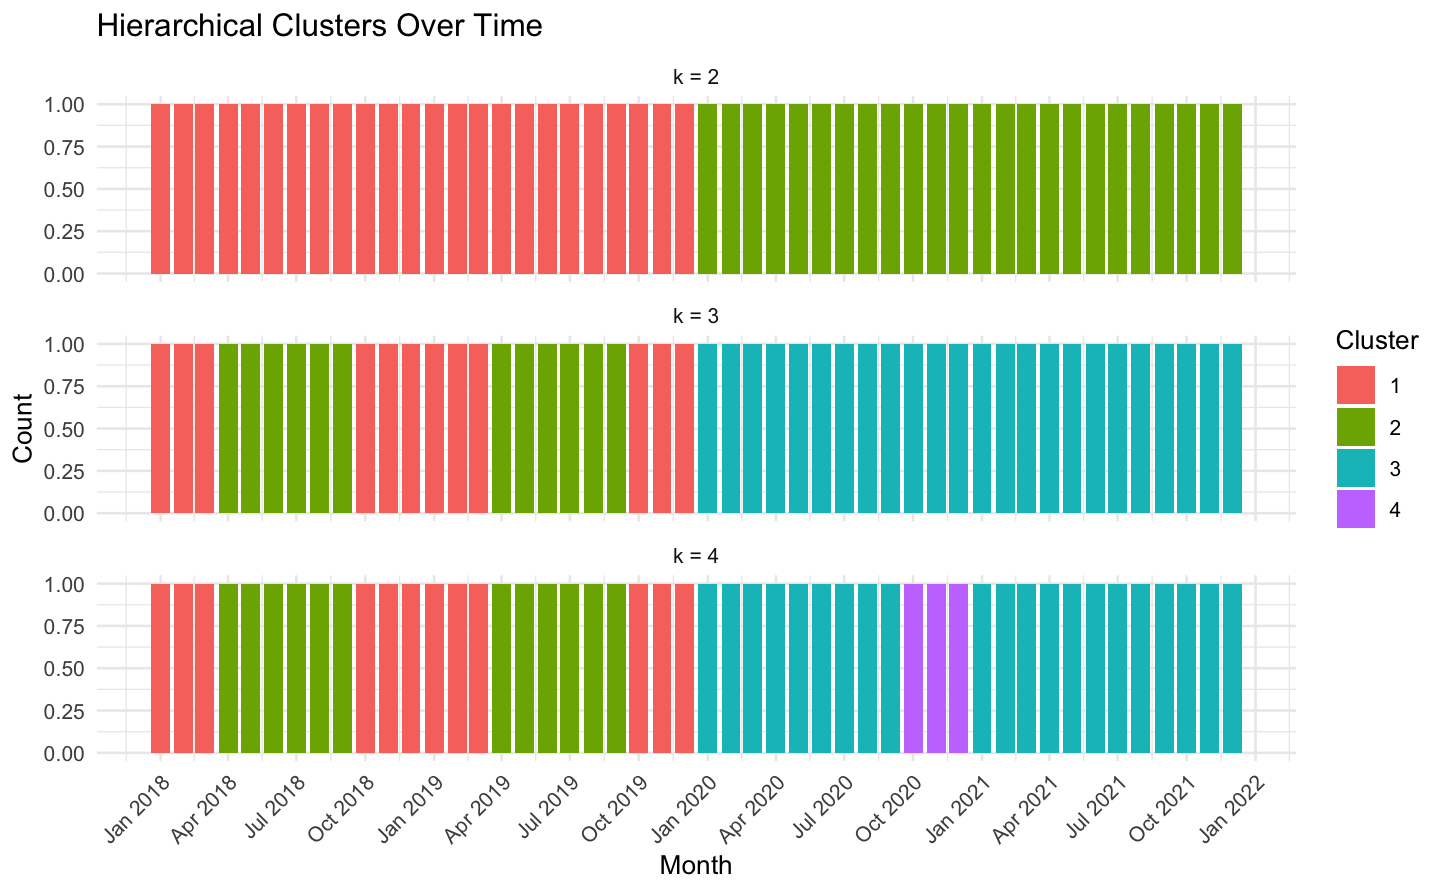
\includegraphics[width=0.75\linewidth]{clr_hierclus.png}
        \caption{Different Clusters of Hiearchical Clustering Method}
        \label{fig:clr_hierclus}
    \end{figure}
\end{frame}

\begin{frame}
   \begin{figure}
       \centering
       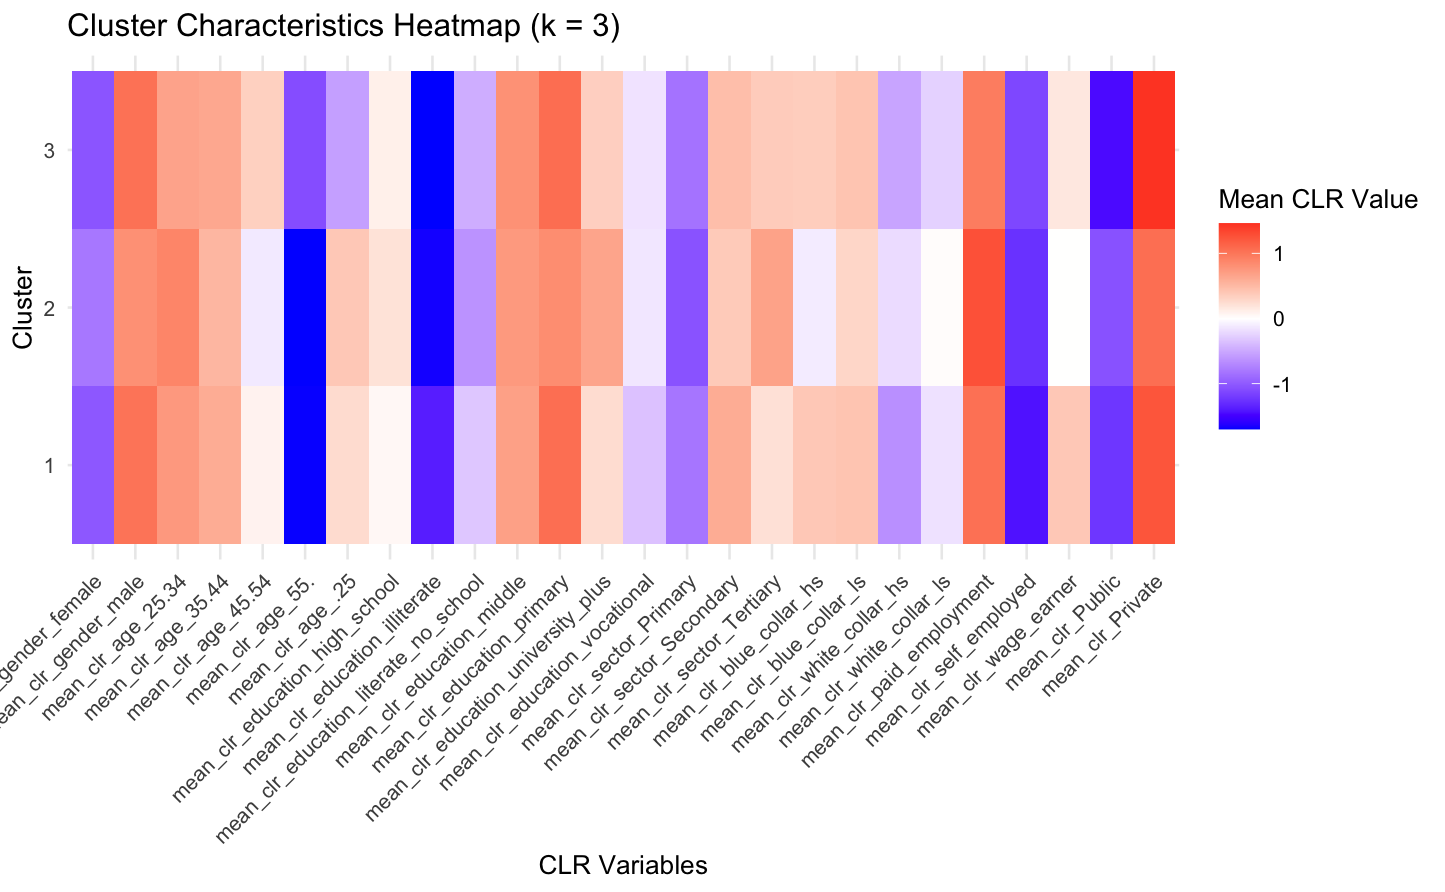
\includegraphics[width=0.75\linewidth]{clr_hier_heatmap.png}
       \caption{Heatmap for k=3}
       \label{fig:clr_hier_heatmap}
   \end{figure}
\end{frame}



\section{Robustness Check}
\begin{frame}
    \frametitle{Robustness Check}
  \begin{figure}
      \centering
      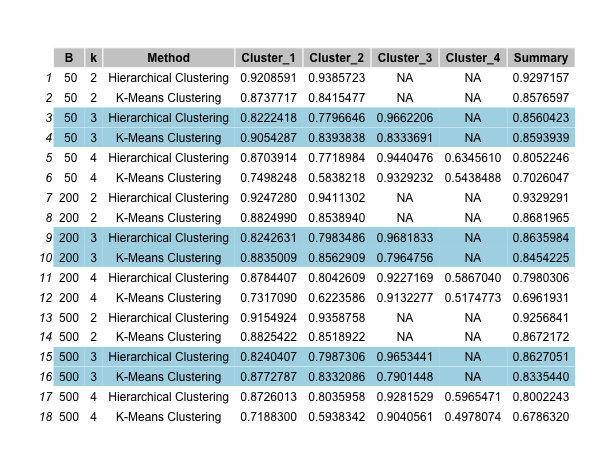
\includegraphics[width=0.7\linewidth]{highlighted_k3_with_cluster4_table}
      \caption{Cluster Stability Analysis via Bootstrapping}
      \label{fig:bootstrap}
  \end{figure}
\end{frame}

\section{Remarks}
\begin{frame}
    \frametitle{Remarks}
\begin{itemize}
\item Our findings are mixed. Some of them are robust in the sense that they are in line with the related literature, some of them are not. This is probably because:
\begin{itemize}
    \item We use \textbf{different data}.
    \item We have more \textbf{data limitations}.    
\end{itemize}
\end{itemize}
    
   
\end{frame}

\begin{frame}{Remarks (cont'd)}
\begin{itemize}
    \item For Age Groups in Unemployment:
    \begin{itemize}
        \item might have been increased for 55+
         \item might have been decreased for 25-
    \end{itemize}
   
    \begin{itemize}
        \item This might be because of the fact that elder people tend to be less skilled and educated.
        \item Younger people got out of the labor force and became inactive, waiting for the pandemic to come to an end. This is commonly hypothesized in the related literature.
    \end{itemize}
    
\end{itemize}
    
\end{frame}

\begin{frame}{Remarks (cont'd)}
    

\begin{itemize}
    \item We see that wage earners and self-employed population suffered more in terms of losing their jobs, which was also suggested by \textcolor{blue}{(Aygün et al. 2021)}
    \item We can say that blue collar workers were affected more than the white collar workers, controlling for in-group skill levels.
\end{itemize}
\end{frame}
\begin{frame}{Remarks (cont'd)}
    \begin{itemize}
        \item Slightly increasing unemployment among female workers at the beginning of COVID, in contrast with \textcolor{blue}{(Aygün et al. 2021)}
        \item As a general trend, blue-collar unemployment was more affected.
        
    \end{itemize}
\end{frame}
\begin{frame}{Remarks (cont'd)}
\begin{itemize}
    \item \textbf{"shecession"} is not significantly recognizable in our findings. This might be because:
    \begin{itemize}
    \item \textbf{Data difference and limitations}
    \item \textbf{We controlled for the persistent labor force.}
        
    \end{itemize}
\end{itemize}

    
\end{frame}

\begin{frame}{Remarks (cont'd)}
\begin{itemize}
    \item Those who had primary, middle and vocational education might have been affected more. \textcolor{blue}{(Montenovo et al. 2020)}  
    \item Clustering analysis presented different outlooks, capturing more sophisticated interrelations.
    
\end{itemize}
    
\end{frame}


\section{References}
\begin{frame}
    \frametitle{References}
    \begin{itemize}
        \item The Effects of COVID-19 on Labor Market Outcomes in Turkey, 2021, Aysun Hiziroglu Aygun, Selin Koksal and Gokce Uysal
        \item Covid 19 and the Turkish labor market: Heterogeneous effects across demographic groups, 2021, Altan Aldan, Muhammet Enes Çıraklı, Huzeyfe Torun
        \item COVID-19 küresel salgınının 2021 yılında Türk işgücü piyasası üzerinde etkileri: Google Hareketlilik ver- ilerini kullanarak bugünü tahmin etme modelinden elde edilen sonuçlar, 2021. ILO
        \item Impact of the COVID-19 Outbreak on Turkey’s Economy and a Policy Alternative for Protecting Labor Incomes, 2020, Ebru Voyvoda, A. Erinç Yeldan
        \item Determinants of Disparities in Covid-19 Job Losses, 2020, Montenovo et al. 2020.
        \item Covid-19'un Ekonomik Etkileri, 2020, Selva Demiralp
    \end{itemize}
    
 
\end{frame}
\begin{itemize}
         \item COVID-19 doesn’t need lockdowns to destroy jobs: The effect of local outbreaks in Korea, 2021, Aum et al.
        \item The Heterogeneous Labor Market Impacts of the COVID-19 Pandemic, 2020, Cortes and Forsythe
        \item Gender Inequality in Paid and Unpaid Work During Covid-19 Times, 2020, Farre et al.
        \item The Effect of COVID-19 as an Economic Shock on the Gender and Ethnic Gap in Labour Market Outcomes, 2021, Milovanska et al.
        \item Work, Care and Gender during the COVID-19 Crisis, 2020, Petrongolo
        \item Measuring Unemployment: A Composition Model, 2015, Jackson
\end{itemize}


\section{Questions}
\begin{frame}
    \frametitle{Our Questions For You :)}
    
   
\end{frame}


\end{document}


